\documentclass[10pt]{article}

\usepackage{amsmath}
\usepackage{amssymb} 

%%% Language setting for (xe|lua)latex %%%
\usepackage{fontspec}
\usepackage[math-style=TeX]{unicode-math}
\setmainfont{CMU Serif}
\setsansfont{CMU Sans Serif}
\setmonofont{CMU Typewriter Text}
\newfontfamily{\cyrillicfonttt}{CMU Serif}
\setmathfont{XITS Math}[math-style=TeX]

\usepackage{polyglossia}
\setdefaultlanguage[spelling=modern]{russian}

\usepackage{cyrmathtext}

\usepackage{hyperref}
\hypersetup{%
	pdfencoding=auto
}

\usepackage{babel}

\usepackage{graphicx}
\usepackage{todonotes}

\begin{document}

\title{Обработка результатов учебного эксперимента}
\begin{abstract}
    Данное пособие содержит краткое изложение основных понятий и методов,
    необходимых для корректной обработки результатов экспериментов в учебной
    лаборатории, а также указания по представлению результатов лабораторных
    работ, с тем чтобы оформленные студентами отчёты в целом соответствовали
    сложившимся современным стандартам оформления научных публикаций.
    
    Умение работать с погрешностями, или <<ошибками>>,
    является важной частью любого научного эксперимента на всех его этапах.
    Так, при подготовке и проведении эксперимента необходимо знать точность
    используемых приборов, уметь находить пути возможного уменьшения ошибок,
    разумно организовать сами измерения и правильно оценивать точность
    полученных значений. На этапе обработки возникает необходимость пересчитывать
    возможную ошибку в конечных результатах по известным оценкам погрешностей
    в исходных данных. А на самом важном этапе --- интерпретации
    результатов эксперимента --- без знания точности проведённых
    измерений и без корректной статистической обработки невозможно делать
    обоснованные выводы в пользу той или иной физической модели, той или
    иной гипотезы. 
    
    Пособие может быть рекомендовано студентам первого курса для первичного
    ознакомления с предметом, либо в качестве <<шпаргалки>>
    по основным формулам. Более подробное изложение материла, снабжённое
    большим количеством практических примеров, пособия можно найти в книгах
    \cite{taylor,squires,zaidel}. Студентам старших курсов, знакомым
    с основами теории вероятностей и математической статистики, и желающим
    изучить материал на более глубоком уровне и познакомиться с <<продвинутыми>>
    современными методиками обработки данных, можно порекомендовать начать
    с книги \cite{hudson}.
\end{abstract}

\maketitle
\tableofcontents

\section{Измерения и погрешности}

\subsection{Результат измерения}

\emph{Результат измерения} --- количественная характеристика
какого-либо физического объекта, явления или процесса. Она получается
из сравнения (прямого или косвенного) измеряемой величины с некоторым
\emph{эталоном}.
\todo[ author= Nozik]{
    Про эталон мне не очень нравится, это очень узкое определение. Потом придумаю что-нибудь более универсальное
}

Для наглядности рассмотрим простейший пример измерения длины стержня
с помощью линейки. Линейка проградуирована производителем с помощью
некоторого эталона длины --- таким образом, сравнивая длину
стержня с ценой деления линейки, мы косвенно сравниваем его с принятым
стандартным эталоном. 

Допустим, мы приложили линейку к стержню и увидели некоторый результат
$x=x_{\text{изм}}$. Что можно сказать о длине стержня?

Во-первых, значение $x$ \emph{не может быть задано точно}, хотя бы
потому, что оно обязательно \emph{округлено} до некоторой значащей
цифры: если линейка <<обычная>>, то у неё
есть \emph{цена деления}; а если линейка, к примеру, <<лазерная>>
--- у неё высвечивается \emph{конечное число значащих цифр}
на дисплее.

Во-вторых, мы никак не можем быть уверенны, что длина стержня \emph{на
самом деле} такова хотя бы с точностью до ошибки округления. Действительно,
мы могли приложить линейку не вполне ровно; сама линейка могла быть
изготовлена не вполне точно; стержень может быть не идеально цилиндрическим
и т.п.

Итак, из нашего примера видно, что физическое измерение не может быть
произведено точно, то есть у любого измерения есть \emph{погрешность}.
\footnote{Также используют эквивалентный термин \emph{ошибка измерения} (от\emph{
англ.} error). Подчеркнём, что смысл этого термина отличается от общеупотребительного
бытового: если физик говорит <<в измерении есть ошибка>>,
--- это не означает, что оно неправильно и его надо переделать.\emph{
}Имеется ввиду лишь, что это измерение \emph{неточно}, то есть имеет
\emph{погрешность}. } 

{\footnotesize{}Количественно погрешность можно было бы попытаться
определить как разность между измеренным и <<истинным>>
значением длины стержня: $\delta x=x_{0}-x_{\text{ист}}$. Однако
такое определение в общем случае }\emph{\footnotesize{}бессмысленно}{\footnotesize{}:
во-первых, раз у }\emph{\footnotesize{}любого}{\footnotesize{} измерения
есть погрешность, значит <<истинное>> значение
измерить }\emph{\footnotesize{}невозможно}{\footnotesize{}, во-вторых,
само <<истинное>> значение может быть }\emph{\footnotesize{}не
определено}{\footnotesize{} вовсе (например, стержень неровный или
изогнутый, его торцы дрожат из-за тепловых флуктуаций и т.д.).}{\footnotesize\par}

По результатам измерения можно говорить о возможном \emph{диапазоне}
значений, в пределах которого может лежать измеряемая величина. Как
правило, результат измерения можно записать как
\[
x=x_{\text{изм}}\pm\delta x,
\]
где $\delta x$ --- \emph{абсолютная величина} погрешности.
Эта запись означает, что исследуемая величина лежит в интервале $x\in(x_{\text{изм}}-\delta x;\,x_{\text{изм}}+\delta x)$
с некоторой достаточно большой долей вероятности. Важной характеристикой
качества измерения является \emph{относительная величина} погрешности
\[
\varepsilon_{x}=\frac{\delta x}{x_{\text{изм}}},
\]
то есть то, насколько погрешность мала по сравнению с самой измеряемой
величиной (как правило, её выражают в процентах, т.е. $\varepsilon=\frac{\delta x}{x}\cdot100\%$).

\textbf{\footnotesize{}Пример.}{\footnotesize{} Штангенциркуль ---
прибор для измерения длин с ценой деления $0{,}1\;\text{мм}$. Пусть
диаметр некоторой проволоки равен $0{,}37$~мм. Считая, что абсолютная
ошибка составляет половину цены деления прибора, результат измерения
можно будет записать как $d=0{,}40\pm0{,}05\;\text{мм}$ (или $d=(40\pm5)\cdot10^{-5}\;\text{м}$).
Относительная погрешность составляет $\varepsilon\approx13\%$, то
есть точность измерения весьма посредственная --- поскольку
размер объекта близок к пределу точности прибора.}{\footnotesize\par}

\paragraph{О необходимости оценки погрешностей.}

Измерим длины двух стержней $x_{1}$ и $x_{2}$ и сравним результаты.
Можно ли сказать, что стержни одинаковы или различны? Казалось бы,
достаточно проверить, справедливо ли $x_{1}=x_{2}$. Но \emph{никакие}
два результата не равны друг другу с абсолютной точностью! Таким образом,
без указания погрешности измерения ответ на этот вопрос дать \emph{невозможно}. 

С другой стороны, если погрешность $\delta x$ известна, то можно
утверждать, что если измеренные длины одинаковы \emph{в пределах погрешности
опыта}, если $|x_{2}-x_{1}|<\delta x$ (и различны в противоположном
случае).

Итак, без знания погрешностей невозможно сравнить между собой никакие
два измерения, и, следовательно, невозможно сделать \emph{никаких}
значимых выводов по результатам эксперимента: ни о наличии зависимостей
между величинами, ни о практической применимости какой-либо теории,
и т.\,п. В связи с этим крайне важной является задача правильной
оценки погрешностей, поскольку её существенное занижение или завышение
(по сравнению с реальной точностью измерений) ведёт к \emph{неправильным
выводам}.

В лабораторном практикуме оценка погрешностей должна проводиться \emph{всегда}
(даже когда составители задания забыли упомянуть об этом).

\subsection{Многократные измерения}

Проведём серию из $n$ \emph{одинаковых (однотипных}) измерений одного
и того же объекта (многократно приложили линейку к стержню) и получим
ряд значений
\[
\left\{ x_{1},\,x_{2},\,\ldots\,,x_{n}\right\} .
\]
Что можно сказать о данном наборе чисел и о длине стержня?

Нетрудно убедиться на практике, что величины $\left\{ x_{i}\right\} $
почти наверняка окажутся \emph{различными}. Причиной тому могут быть
самые разные обстоятельства, например: у нас недостаточно остроты
зрения и точности рук, чтобы каждый раз прикладывать линейку одинаково;
стенки стержня могут быть слегка неровными; у стержня может и не быть
определённой длины, например, если в нём возбуждены звуковые волны,
из-за чего его торцы колеблются, и т.\,д.

Итак, результаты серии измерений являются \emph{случайными величинами}.
Поэтому для их анализа и обработки можно применять методы теории вероятностей
и математической статистики.

Если методика измерения достаточно надёжна, а объект измерения достаточно
стабилен (стержень не расплывается, как облако на ветру), то можно
ожидать, что разброс значений $\left\{ x_{i}\right\} $ невелик и
почти все результаты находятся в ограниченном диапазоне вблизи некоторого
среднего. Обозначим среднее по результатам $n$ измерений как $\overline{x}$
и определим его как \emph{среднее арифметическое}:
\begin{equation}
\overline{x}=\frac{x_{1}+x_{2}+\ldots+x_{n}}{n}\equiv\frac{1}{n}\sum\limits _{i=1}^{n}x_{i}\label{eq:average}
\end{equation}
(в математической статистике его называют \emph{выборочным средним}).

Пусть число измерений велико: $n\gg1$. Если сказанное о стабильности
прибора, методики и объекта измерения верно, можно ожидать, что сумма
(\ref{eq:average}) будет стремиться к некоторому пределу\footnote{В теории вероятностей факт существования данного предела называют
\emph{законом больших чисел}. Он выполняется при достаточно общих
предположениях о характере случайной величины $x$. Тем не менее,
в некоторых случаях этот предел может и не существовать. Такие ситуации
требуют особого рассмотрения и мы на них не останавливаемся.}:
\[
\lim_{n\to\infty}\frac{1}{n}\sum_{i=1}^{n}x_{i}=x_{0}.
\]
Предельное значение $x_{0}$ можно условно назвать <<истинным>>
средним для данной случайной величины.

\todo[author = Nozik, inline]{Ну вот тут получается  странность, здесь совсем упрощенное изложение, при этом позже есть нормальное изложение теории вероятностей. По-моему надо все-таки сначала рассказать, что такое распределение, и потом от этого плясать, а не пытаться извернуться с описанием на пальцах}

<<Разброс>> данных можно характеризовать
отклонением результатов от среднего:
\[
\Delta x_{i}=x_{i}-\overline{x},\qquad i=1\ldots n.
\]
(не путать с погрешностью каждого измерения $\delta x_{i}$!). В частности,
можно было бы определить максимальное по модулю отклонение $\left|\Delta x\right|_{\mathrm{max}}$:
все измерения лежат в диапазоне $\overline{x}-\left|\Delta x\right|_{\mathrm{max}}\le x\le\overline{x}+\left|\Delta x\right|_{\mathrm{max}}$.
Однако с математической точки зрения работать с модулем неудобно,
поэтому на практике используется \emph{средняя квадратичная} величина
отклонения (точнее, её выборочное значение):
\begin{equation}
s_{x}=\sqrt{\frac{\Delta x_{1}^{2}+\Delta x_{2}^{2}+\ldots+\Delta x_{n}^{2}}{n}}=\sqrt{\frac{1}{n}\sum\limits _{i=1}^{n}\Delta x_{i}^{2}}\label{eq:sigma}
\end{equation}
или кратко
\begin{equation}
\boxed{s_{x}^{2}=\overline{\left(x-\overline{x}\right)^{2}}}.\label{eq:sigma_s}
\end{equation}
Квадрат $s_{x}^{2}$ принято называть (выборочной) \emph{дисперсией}
случайной величины. Предельную величину среднеквадратичного отклонения
при $n\to\infty$ обозначим как
\[
\sigma_{x}=\lim\limits _{n\to\infty}s_{x}.
\]

Как правило, б\'ольшая часть измерений (какая именно ---
обсудим позже) находится в диапазоне $\overline{x}-\sigma_{x}<x<\overline{x}+\sigma_{x}.$

{\footnotesize{}Отметим одну полезную формулу для дисперсии. Пользуясь
тем, что среднее от суммы равно сумме средних, и раскрывая скобки
в определении (\ref{eq:sigma_s}), найдём
\begin{equation}
s_{x}^{2}=\overline{\left(x-\overline{x}\right)^{2}}=\overline{x^{2}-2x\overline{x}+\overline{x}^{2}}=\overline{x^{2}}-\overline{x}^{2},\label{eq:sigma_x2}
\end{equation}
то есть дисперсия равна разности среднего значения квадрата $\overline{x^{2}}=\frac{1}{n}\sum\limits _{i=1}^{n}x_{i}^{2}$
и квадрата среднего $\overline{x}^{2}=\left(\frac{1}{n}\sum\limits _{i=1}^{n}x_{i}\right)^{2}$.}{\footnotesize\par}

\subsection{Классификация погрешностей}

Можно ли улучшить результаты опыта, повторяя его многократно? Будет
ли среднее значение $\overline{x}$ <<лучше>>,
чем каждое измерение $x_{i}$ в отдельности? Чтобы ответить на эти
вопросы, проанализируем источники и виды погрешностей.

В первую очередь, многократное повторение опыта позволяет проверить
\emph{воспроизводимость} результатов: повторные измерения в \emph{одинаковых}
условиях, должны давать близкие результаты\footnote{Невоспроизводимые явления исследовать, очевидно, невозможно. Например,
мы почти ничего не знаем об устройстве <<шаровой молнии>>,
поскольку ещё никому не удалось создать стабильные условия для её
получения, хотя свидетельства существования этого редкого атмосферного
явления довольно многочисленны и надёжны.}. Таким образом, многократные измерения \emph{необходимы} для того,
чтобы убедиться как в надёжности методики, так и в существовании измеряемой
величины как таковой.

При любых измерениях возможны грубые ошибки --- \emph{промахи}
(\emph{англ.} miss). Это <<ошибки>> в стандартном
понимании этого слова --- возникающие по вине экспериментатора
или в силу других непредвиденных обстоятельств, например, из-за сбоя
аппаратуры. Промахов, конечно, нужно избегать, а результаты таких
измерений должны быть по возможности исключены из рассмотрения. Как
понять, является ли <<аномальный>> результат
промахом? Вопрос этот весьма непрост. В литературе существуют статистические
критерии отбора промахов, которыми мы, однако, настоятельно не рекомендуем
пользоваться (по крайней мере, без серьезного понимания последствий
такого отбора). Отбрасывание аномальных данных может, во-первых, привести
к тенденциозному искажению результата исследований, а во-вторых, так
можно упустить открытие неизвестного эффекта. Поэтому при научных
исследованиях необходимо максимально тщательно проанализировать причину
каждого промаха, в частности, многократно повторив эксперимент\footnote{Надо заметить, что это всё равно не даёт полной защиты от промахов,
ведь порой \emph{весь эксперимент} может оказаться одним большим <<промахом>>
(из недавних примеров можно вспомнить <<открытие>>
сверхсветовых нейтрино). Самый радикальный способ проверки достоверности
результатов --- многократная независимая проверка на других
приборах, другими методами, и желательно, другими экспериментаторами.}. Лишь только если факт и причина промаха установлены вполне достоверно,
соответствующий результат можно отбросить.

При многократном повторении измерении одной и той же физической величины
погрешности могут иметь \emph{систематический} либо \emph{случайный}
характер. Назовём погрешность \emph{систематической}, если она повторяется
от опыта к опыту, сохраняя свой знак и величину, либо \emph{закономерно}
меняется в процессе измерений. \emph{Случайные} (или \emph{статистические})
погрешности меняются хаотично при повторении измерений как по величине,
так и по знаку, и в изменениях не прослеживается какой-либо закономерности.

Кроме того, удобно разделять погрешности по их происхождению. Можно
выделить
\begin{itemize}
\item \emph{инструментальные} (или \emph{приборные}) \emph{погрешности},
связанные с несовершенством конструкции (неточности, допущенные при
изготовлении или вследствие старения), ошибками калибровки или ненормативными
условиями эксплуатации измерительных приборов;
\item \emph{методические} \emph{погрешности}, связанные с несовершенством
теоретической модели явления (использование приближенных формул и
моделей явления) или с несовершенством методики измерения (например,
влиянием взаимодействия прибора и объекта измерения на результат измерения);
\item \emph{естественные} \emph{погрешности}, связанные со случайным характером
измеряемой физической величины --- они являются не столько
<<ошибками>> измерения, сколько характеризуют
природу изучаемого объекта или явления.
\end{itemize}
{\footnotesize{}Разделение погрешностей на систематические и случайные
не является однозначным и зависит от постановки опыта. Например, производя
измерения не одним, а несколькими однотипными приборами, мы переводим
систематическую приборную ошибку, связанную с неточностью шкалы и
калибровки, в случайную. Разделение по происхождению также условно,
поскольку любой прибор подвержен воздействию <<естественных>>
случайных и систематических ошибок (шумы и наводки, тряска, атмосферные
условия и т.\,п.), а в основе работы прибора всегда лежит некоторое
физическое явление, описываемое не вполне совершенной теорией.}{\footnotesize\par}

\subsubsection{Случайные погрешности}

Случайный характер присущ большому количеству различных физических
явлений и в той или иной степени проявляется в работе всех без исключения
приборов. Случайные погрешности обнаруживаются просто при многократном
повторении опыта --- в виде хаотичных изменений (\emph{флуктуаций})
значений $\left\{ x_{i}\right\} $.

Если случайные отклонения от среднего в большую или меньшую стороны
примерно равновероятны, можно рассчитывать, что при вычислении среднего
арифметического (\ref{eq:average}) эти отклонения скомпенсируются,
и погрешность результирующего значения $\overline{x}$ будем меньше,
чем погрешность отдельного измерения.

Случайные погрешности бывают связаны, например,

1. \emph{с особенностями используемых приборов}: техническими недостатками
(люфт в механических приспособлениях, сухое трение в креплении стрелки
прибора), с естественными (тепловой и дробовой шумы в электрических
цепях, тепловые флуктуации и колебания измерительных устройств из-за
хаотического движения молекул, космическое излучение) или техногенными
факторами (тряска, электромагнитные помехи и наводки);

2. \emph{с особенностями и несовершенством методики измерения} (ошибка
при отсчёте по шкале, ошибка времени реакции при измерениях с секундомером);

3. \emph{с несовершенством объекта измерений} (неровная поверхность,
неоднородность состава);

4. \emph{cо случайным характером исследуемого явления} (радиоактивный
распад, броуновское движение).

Остановимся несколько подробнее на двух последних случаях. Они отличаются
тем, что случайный разброс данных в них порождён непосредственно объектом
измерения. Если при этом приборные погрешности малы, то <<ошибка>>
эксперимента возникает лишь в тот момент, когда мы \emph{по своей
воле} совершаем замену ряда измеренных значений на некоторое среднее
$\left\{ x_{i}\right\} \to\overline{x}$. Разброс данных при этом
характеризует не точность измерения, а сам исследуемый объект или
явление. Однако с \emph{математической} точки зрения приборные и <<естественные>>
погрешности \emph{неразличимы} --- глядя на одни только
экспериментальные данные невозможно выяснить, что именно явилось причиной
их флуктуаций: сам объект исследования или иные, внешние причины.
Таким образом, для исследования естественных случайных процессов необходимо
сперва отдельно исследовать и оценить случайные инструментальные погрешности
и убедиться, что они достаточно малы.

\subsubsection{Систематические погрешности}

Систематические погрешности, в отличие от случайных, невозможно обнаружить,
исключить или уменьшить просто многократным повторением измерений.
Они могут быть обусловлены, во-первых, неправильной работой приборов
(\emph{инструментальная погрешность}), например, cдвигом нуля отсчёта
по шкале, деформацией шкалы, неправильной калибровкой, искажениями
из-за не нормативных условий эксплуатации, искажениями из-за износа
или деформации деталей прибора, изменением параметров прибора во времени
из-за нагрева и т.п. Во-вторых, их причиной может быть ошибка в интерпретации
результатов (\emph{методическая погрешность}), например, из-за использования
слишком идеализированной физической модели явления, которая не учитывает
некоторые значимые факторы (так, при взвешивании тел малой плотности
в атмосфере необходимо учитывать силу Архимеда; при измерениях в электрических
цепях может быть необходим учет неидеальности амперметров и вольтметров
и т.\,д.).

Систематические погрешности условно можно разделить на следующие категории.

1. Известные погрешности, которые могут быть достаточно точно вычислены
или измерены. При необходимости они могут быть учтены непосредственно:
внесением поправок в расчётные формулы или в результаты измерений.
Если они малы, их можно отбросить, чтобы упростить вычисления.

2. Погрешности известной природы, конкретная величина которых неизвестна,
но максимальное значение вносимой ошибки может быть определено теоретически
или экспериментально. Такие погрешности неизбежно присутствуют в любом
опыте, и задача экспериментатора --- свести их к минимуму,
совершенствуя методики измерения и выбирая более совершенные приборы.

Чтобы оценить величину систематических погрешностей опыта, необходимо
учесть паспортную точность приборов (производитель, как правило, гарантирует,
что погрешность прибора не превосходит некоторой величины), проанализировать
особенности методики измерения, и по возможности, провести контрольные
опыты.

3. Погрешности известной природы, оценка величины которых по каким-либо
причинам затруднена (например, сопротивление контактов при подключении
электронных приборов). Такие погрешности должны быть обязательно исключены
посредством модификации методики измерения или замены приборов.

4. Наконец, нельзя забывать о возможности существования ошибок, о
которых мы не подозреваем, но которые могут существенно искажать результаты
измерений. Такие погрешности самые опасные, а исключить их можно только
многократной \emph{независимой} проверкой измерений, разными методами
и в разных условиях.

В учебном практикуме учёт систематических погрешностей ограничивается,
как правило, паспортными погрешностями приборов и теоретическими поправками
к упрощенной модели исследуемого явления.

\section{Основы статистической обработки измерений}

\todo[inline, author = Nozik]{Вот это надо в начало!}

Предположим, что систематические погрешности малы и займёмся отдельно
изучением случайных погрешностей. Пусть по результатам многократных
измерений получен набор значений $\left\{ x_{i}\right\} $, вычислено
их среднее (\ref{eq:average}) $\overline{x}$ и среднеквадратичное
отклонение (\ref{eq:sigma}) $\sigma_{x}\approx s{}_{x}$. Можно надеяться,
что измеряемая величина лежит в диапазоне
\[
x\in\left(\overline{x}-\sigma_{x};\,\overline{x}+\sigma_{x}\right).
\]
Какова вероятность $P$ того, что результат действительно находится
в указанном интервале?

Для ответа на этот вопрос необходимо знать \emph{вероятностный закон},
которому подчиняется исследуемая величина. Казалось бы, для каждой
случайной физической величины должен существовать свой особенный закон
и общую теорию здесь построить невозможно. Это отчасти верно, но оказывается,
что существует вполне \emph{универсальный} вероятностный закон, называемый
\emph{нормальным}, которому подчиняются многие случайные величины.
Рассмотрим его подробнее.

\subsection{Нормальный закон распределения}

\todo[inline, author = Nozik]{Нормальное распределение вводится без объяснения того, что такое распределение!}

Одним из наиболее примечательных результатов теории вероятностей является
так называемая \emph{центральная предельная теорема}, которая утверждает,
что сумма большого количества независимых случайных слагаемых, каждое
из которых вносит в эту сумму относительно малый вклад, подчиняется
универсальному закону, не зависимо от того, каким вероятностным законам
подчиняются её составляющие, --- так называемому \emph{нормальному
распределению} (или \emph{распределению Гаусса}). Эта теорема имеет
прямое отношение к физическим измерениям, поскольку зачастую случайные
погрешности складываются из множества случайных \emph{независимых}
факторов.

Доказательство теоремы довольно сложно и мы его не приводим. Остановимся
кратко на том, что такое нормальное распределение и его основных свойствах.

\paragraph{Гистограмма.}

Построим примерную \emph{гистограмму} для результатов серии $n$ измерений.
Область значений $x$, размещённую на оси абсцисс, разобьём на равные
малые интервалы --- <<корзины>>
или <<бины>> (\emph{англ.} bins) некоторого
размера $h$. По оси ординат будет откладывать долю измерений $w$,
результаты которых попадают в соответствующую корзину. Например, если
$n_{k}$ измерений лежит в диапазоне $kh<x<(k+1)h$, $k$ ---
номер корзины, то на графике изобразим столбик шириной $h$ и высотой
$w_{k}=n_{k}/n$. В результате получим картину, подобную изображённой
на рис.~\ref{fig:normhist}. Самые высокие столбики будут сосредоточены
вблизи среднего $\overline{x}$; ширина гистограммы будет по порядку
величины равна $\sigma$, а при отклонении от $\overline{x}$ на несколько
$\sigma$ столбиков не будет совсем.

\begin{figure}
\begin{centering}
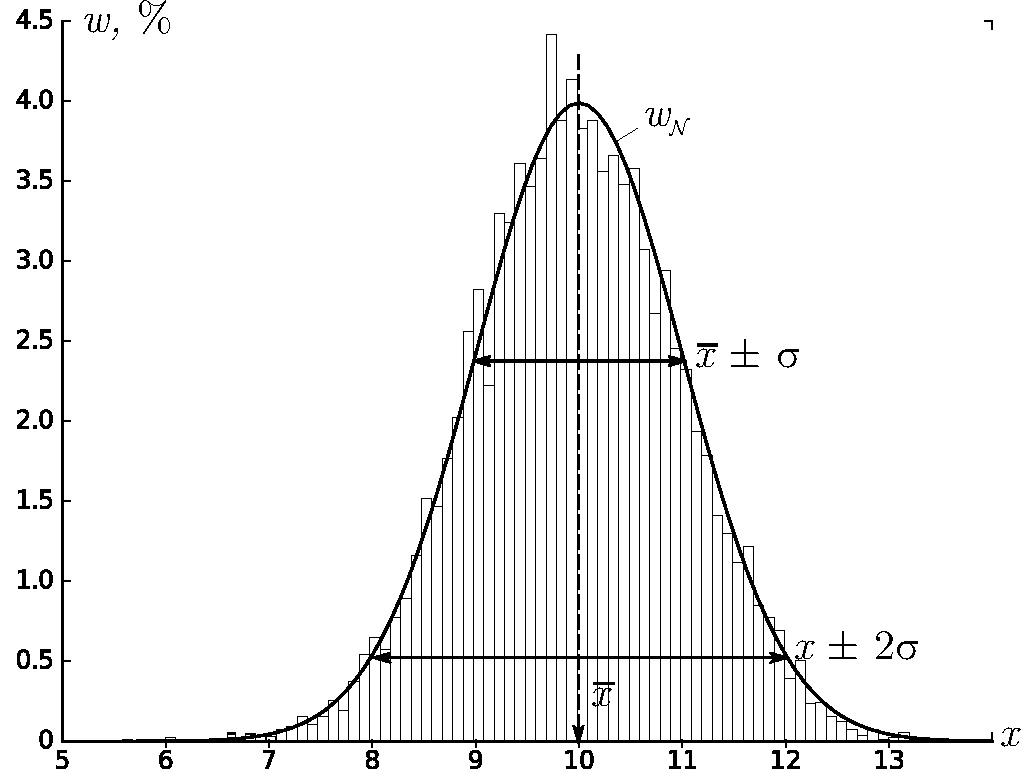
\includegraphics[width=7cm,bb = 0 0 200 100, draft, type=eps]{normhist.pdf}
\par\end{centering}
\caption{\label{fig:normhist}Пример гистограммы для нормального распределения
($\overline{x}=10$, $\sigma=1{,}0$, $h=0{,}1$, $n=10^{4}$)}
\end{figure}


\paragraph{Плотность распределения.}

Какова будет форма гистограммы в пределе $n\to\infty$? Оказывается,
что если выполнены описанные выше предпосылки центральной предельной
теоремы, то её огибающая будет описываться функцией
\begin{equation}
\boxed{w_{\mathcal{N}}\!\left(x\right)=\frac{1}{\sqrt{2\pi}\sigma}e^{-\tfrac{(x-x_{0})^{2}}{2\sigma^{2}}}},\label{eq:normal}
\end{equation}
которую называют \emph{плотностью нормального распределения}, или
просто \emph{нормальным распределением}. Здесь $x_{0}$ и $\sigma$
--- параметры нормального распределения: $x_{0}$ равно
среднему (и наиболее вероятному) значению $x$, a $\sigma$ ---
среднеквадратичному отклонению, вычисленным в пределе $n\to\infty$. 

Если необходимо найти долю измерений (вероятность), дающих результат
в интервале $x\in\left[a;b\right]$, нужно вычислить площадь под графиком
функции $w\!\left(x\right)$ в пределах $a\le x\le b$:
\begin{equation}
    P_{a\le x\le b}=\int\limits _{a}^{b}w\!\left(x\right)dx.\label{eq:P}
\end{equation}

Как видно из рис. 1, распределение представляет собой симметричный
<<колокол>>, положение вершины которого
соответствует среднему значению $\bar{x}$ (ввиду симметрии, оно же
совпадает с наиболее вероятным значением --- максимумом
функции $w_{\mathcal{N}}(x)$).

\begin{figure}
%    \centering\input{gauss.pdf_t}
    \caption{Плотность нормального распределения}
\end{figure}

Полная площадь под графиком есть суммарная доля всех возможных случаев,
то есть равна единице: $\int\limits _{-\infty}^{\infty}w\left(x\right)dx=1$.
Это соотношение называют \emph{условием нормировки}. 

При значительном отклонении $x$ от среднего величина $w_{\mathcal{N}}\!\left(x\right)$
быстро убывает. Это означает, что вероятность встретить отклонения,
существенно большие, чем $\sigma$, оказывается \emph{пренебрежимо
мала}. Ширина <<колокола>> по порядку величины
равна $\sigma$ --- она характеризует <<разброс>>
экспериментальных данных относительно среднего значения.

{\footnotesize{}А именно, точки $x=\bar{x}\pm\sigma$ являются точками
перегиба графика $w\left(x\right)$ (в них вторая производная по $x$
обращается в нуль, $w''=0$), а их положение по высоте составляет
$w\!\left(\bar{x}\pm\sigma\right)/w(\bar{x})=e^{_{-1/2}}\approx0{,}61$
от высоты вершины.}{\footnotesize\par}

Универсальный характер центральной предельной теоремы позволяет широко
применять на практике нормальное (гауссово) распределение для обработки
случайных погрешностей. Заметим, что на практике для \emph{приближённой
оценки} параметров нормального распределения случайной величины используются
\emph{выборочные} значения среднего и дисперсии: $x_{0}\approx\overline{x}$,
$s_{x}\approx\sigma_{x}$.

\subsection{Доверительная вероятность и доверительный интервал}

Обозначим через $P\!\left(\left|\Delta x\right|<\delta\right)$ вероятность
(долю случаев) того, что отклонение от среднего $\Delta x=x-x_{0}$
составит величину, не превосходящую по модулю значение $\delta$:
\[
P\left(\left|\Delta x\right|<\delta\right)=\int\limits _{x_{0}-\delta}^{x_{0}+\delta}w\!\left(x\right)dx.
\]
Величину $P$ называют \emph{доверительной вероятностью} для \emph{доверительного
интервала} $\left|x-x_{0}\right|\le\delta$. 

Для нормального распределения доверительные вероятности могут быть
легко найдены численно\footnote{Заметим, что интеграл $\int e^{-x^{2}/2}dx$, называемый \emph{интегралом
ошибок}, в элементарных функциях не выражается.}. Вероятность отклонения в пределах $\pm\sigma$ оказывается равна
\[
P\!\left(\left|\Delta x\right|<\sigma\right)\approx0{,}68,
\]
в пределах $\pm2\sigma$:
\[
P\!\left(\left|\Delta x\right|<2\sigma\right)\approx0{,}95,
\]
а в пределах $\pm3\sigma$:
\[
P\left(\left|\Delta x\right|<3\sigma\right)\approx0{,}9973.
\]
Таким образом, при большом числе измерений нормально распределённой
величины можно ожидать, например, что 68\% измерений попадут в интервал
$\left[\bar{x}-\sigma;\bar{x}+\sigma\right]$. При этом около 5\%
измерений выпадут за пределы $\left[\bar{x}-2\sigma;\bar{x}+2\sigma\right]$,
и лишь 0,27\% окажутся за пределами $\left[\bar{x}-3\sigma;\bar{x}+3\sigma\right]$.
Вероятность ещё больших отклонений очень быстро убывает\footnote{В сообщениях об открытии бозона Хиггса на Большом адронном коллайдере
говорилось о том, что исследователи ждали подтверждение результатов
с точностью <<5 сигма>>, ---
это означает, что они использовали доверительную вероятность $P\approx1-5{,}7\cdot10^{-7}=0{,}99999943$.
Такую точность можно назвать фантастической.}.

Полученные значения доверительных вероятностей используются при \emph{стандартной
записи результатов измерений}. В физических измерениях (в частности,
в учебной лаборатории), как правило, используется $P=0{,}68$, то
есть, запись 
\[
x=\bar{x}\pm\delta x
\]
означает, что измеренное значение лежит в диапазоне (доверительном
интервале) $x\in\left[\bar{x}-\delta x;\bar{x}+\delta x\right]$ с
вероятностью 68\%. Таким образом погрешность $\pm\delta x$ считается
равной одному среднеквадратичному отклонению: $\delta x=\sigma$.
В технических измерениях чаще используется $P=0{,}95$, то есть под
абсолютной погрешностью имеется в виду удвоенное среднеквадратичное
отклонение, $\delta x=2\sigma$. Во избежание разночтений доверительную
вероятность следует указывать отдельно.

\paragraph{Сравнение результатов измерений.}

Теперь мы можем дать количественный критерий для сравнения двух измеренных
величин или двух результатов измерения одной и той же величины.

Пусть величины $x_{1}$ и $x_{2}$ ($x_{1}\ne x_{2}$) измерены с
погрешностями $\sigma_{1}$ и $\sigma_{2}$ соответственно. 

Рассмотрим сперва случай, когда одна из величин известна с существенно
большей точностью: $\sigma_{2}\ll\sigma_{1}$ (например, $x_{1}$
--- результат, полученный студентом в лаборатории, $x_{2}$
--- справочное значение). Ясно, что если $\left|x_{1}-x_{2}\right|\gg\sigma_{1}$
то результаты заведомо не совпадают, а если $\left|x_{1}-x_{2}\right|\lesssim\sigma_{1}$,
то различия между ними можно объяснить случайным отклонением.

Поскольку $\sigma_{2}$ мало, значение $x_{2}$ можно принять за <<истинное>>
среднее и предположить, что погрешность измерения $x_{1}$ подчиняется
нормальному закону (со средним $x_{2}$ и дисперсией $\sigma_{1}^{2}$).
Тогда с помощью функции (\ref{eq:normal}) можно вычислить вероятность
$P\left(\left|x_{1}-x_{2}\right|\right)$ того, что отклонение $\left|x_{1}-x_{2}\right|$
возникло исключительно в силу случайных причин. Предварительно необходимо
договориться о том, какую вероятность отклонения следует считать \emph{значимой}.
Универсального значения здесь быть не может, поэтому приходится полагаться
на субъективный выбор конкретного исследователя. Часто в качестве
границы выбирают вероятность $P=0{,}05$, то есть результаты признаются
различными, если вероятность случайного отклонения меньше 5\%, и совпадающими
в противоположном случае. Как следует из свойств нормального распределения,
рассмотренных выше, такая вероятность соответствует отклонению на
$2\sigma$, то есть различие значимо, если 
\[
\left|x_{1}-x_{2}\right|>2\sigma_{1}.
\]

Пусть теперь погрешности двух измерений сравнимы по порядку величины,
$\sigma_{1}\sim\sigma_{2}$. В теории вероятностей показывается, что
линейная комбинация нормально распределённых величин также имеет нормальное
распределение. Следовательно, разность $x_{1}-x_{2}$ распределена
нормально с дисперсией $\sigma^{2}=\sigma_{1}^{2}+\sigma_{2}^{2}$
(см. также правила сложения погрешностей (\ref{eq:sigma_sum})). Тогда
для проверки гипотезы о том, что $x_{1}$ и $x_{2}$ являются измерениями
одной и той же величины, нужно вычислить, является ли значимым отклонение
$\left|x_{1}-x_{2}\right|$ от нуля.

\textbf{\footnotesize{}Пример.}{\footnotesize{} Два студента получили
следующие значения для теплоты испарения некоторой жидкости: $x_{1}=40{,}3\pm0{,}2$
кДж/моль и $x_{2}=41{,}0\pm0{,}3$ кДж/моль, где погрешность соответствует
одному стандартному отклонению. Можно ли утверждать, что они исследовали
одну и ту же жидкость?}{\footnotesize\par}

{\footnotesize{}Имеем наблюдаемую разность $\left|x_{1}-x_{2}\right|=0{,}7$,
среднеквадратичное отклонение для разности $\sigma=\sqrt{0{,}2^{2}+0{,}3^{2}}=0{,}36$.
Их отношение $\frac{\left|x_{2}-x_{1}\right|}{\sigma}\approx2$. Из
свойств нормального распределения находим вероятность того, что измерялась
одна и та же величина, а различия в ответах возникли из-за случайных
ошибок: $P\approx5\%$. Ответ на вопрос, <<достаточно>>
ли мала или велика эта вероятность остаётся на усмотрение исследователя.}{\footnotesize\par}

\textbf{\footnotesize{}Замечание.}{\footnotesize{} Изложенные здесь
соображения применимы, только если измеренное значение $x$ и его
стандартное отклонение $\sigma$ получены на основании достаточно
большой выборки $n\gg1$ (или заданы точно). Если приходится иметь
дело с небольшим количеством измерений ($n\lesssim10$), выборочные
средние и стандартные отклонения сами имеют довольно большую погрешность.
Тогда отклонения выборочных величин будут описываться не нормальным
распределением, а так называемым $t$-распределением Стъюдента. В
частности, в зависимости от значения $n$ интервал $\overline{x}\pm s_{x}$
будет соответствовать несколько меньшей доверительной вероятности,
чем $P=0{,}68$. Особенно резко различия проявляются при высоких уровнях
доверительных вероятностей $P\to1$. Подробнее об этом см. {[}?{]}.}{\footnotesize\par}

\subsection{Независимые случайные величины. Корреляция}

Рассмотрим две физические величины $x$ и $y$. Величины называют
\emph{независимыми} если результат измерения одной из них никак не
влияет на результат измерения другой.

Обозначим отклонения от средних как $\Delta x=x-\overline{x}$ и $\Delta y=y-\overline{y}$.
Средние значения отклонений равны, очевидно, нулю: $\overline{\Delta x}=x-\overline{x}=0$,
$\overline{\Delta y}=0$. Из независимости величин $x$ и $y$ следует,
что среднее значение от произведения $\overline{\Delta x\cdot\Delta y}$
равно произведению средних $\overline{\Delta x}\cdot\overline{\Delta y}$
и, следовательно, равно нулю: 
\begin{equation}
\overline{\Delta x\cdot\Delta y}=\overline{\Delta x}\cdot\overline{\Delta y}=0.\label{eq:indep}
\end{equation}

Если $x$ и $y$ не являются независимыми, среднее значение произведения
их отклонений может быть использовано как количественная мера их зависимости.
Наиболее употребительной мерой зависимости двух случайных величин
является \emph{коэффициент линейной корреляции}:
\begin{equation}
r_{xy}=\frac{\overline{\Delta x\cdot\Delta y}}{\sigma_{x}\cdot\sigma_{y}}.\label{eq:pearson}
\end{equation}
Нетрудно проверить (с помощью неравенства Коши\textendash Буняковского),
что $-1\le r\le1$. В частности, для полностью независимых величин
коэффициент корреляции равен нулю, $r=0$, а для линейно зависимых
$y=kx+b$ нетрудно получить $r=1$ при $k>0$ и $r=-1$ при $k<0$.
Примеры промежуточных случаев представлены на рис. TODO.

Если коэффициент $r_{xy}$ близок к единице, говорят, что величины
\emph{коррелируют} между собой (от \emph{англ.} correlate ---
находиться в связи).

\paragraph{Отсутствие корреляции $\protect\not\Rightarrow$ независимость.}

{\small{}Отметим, что (\ref{eq:indep}) --- необходимое,
но не достаточное условие независимости величин. На рис. TODO приведён
пример очевидно зависимых $x$ и $y$, для которых $r\approx0$.}{\small\par}

\paragraph{Корреляция $\protect\not\Rightarrow$ причинность.}

{\small{}Ещё одна типичная ошибка --- исходя из большого
коэффициента корреляции ($r\to1$) между двумя величинами сделать
вывод о функциональной (причинной) связи между $x$ и $y$. Рассмотрим
конкретный пример. Между током и напряжением на некотором резисторе
имеет место линейная зависимость $U=IR$, и коэффициент корреляции
$r_{UI}$ действительно равен единице. Однако }\emph{\small{}обратное
в общем случае неверно}{\small{}. Например, ток в резисторе коррелирует
с его температурой $T$, $r_{IT}\to1$ (больше ток --- больше
тепловыделение по закону Джоуля\textendash Ленца), однако ясно, что
нагрев резистора извне не приведёт к повышению тока в нём (скорее
наоборот, так как сопротивление металлов с температурой растёт). Ошибка
отождествления корреляции и причинности особенно характерна при исследовании
сложных многофакторных систем, например, в медицине, социологии и
т.п.}{\small\par}

\subsection{Сложение случайных погрешностей\label{subsec:sum}}

\todo[inline, author = Nozik]{Частично дублирует то, что уже было}

Пусть измеряемая величина $z=x+y$ складывается из двух \emph{независимы}х
случайных слагаемых $x$ и $y$, для которых известны средние значения
$\overline{x}$ и $\overline{y}$, и их среднеквадратичные погрешности
$\sigma_{x}$ и $\sigma_{y}$. Непосредственно из определения (\ref{eq:average})
следует вполне очевидный результат, что среднее суммы равно сумме
средних: 
\[
\overline{z}=\overline{x}+\overline{y}.
\]

Найдём дисперсию $\sigma_{z}^{2}$. В силу независимости имеем
\[
\overline{\Delta z^{2}}=\overline{\Delta x^{2}}+\overline{\Delta y^{2}}+2\overline{\Delta x\cdot\Delta y}=\overline{\Delta x^{2}}+\overline{\Delta y^{2}},
\]
то есть:
\begin{equation}
\boxed{{\sigma_{x+y}=\sqrt{\sigma_{x}^{2}+\sigma_{y}^{2}}}}.\label{eq:sigma_sum}
\end{equation}
Таким образом, при сложении \emph{независимых }величин их погрешности
складываются среднеквадратичным образом.

Подчеркнём, что для справедливости соотношения (\ref{eq:sigma_sum})
величины $x$ и $y$ не обязаны быть нормально распределёнными ---
достаточно существования конечных значений их дисперсий (однако можно
показать, что если $x$ и $y$ распределены нормально, нормальным
будет и распределение их суммы).

\textbf{\footnotesize{}Замечание.}{\footnotesize{} Требование независимости
слагаемых является принципиальным. Например, положим $y=x$. Тогда
$z=2x$. Здесь $y$ и $x$, очевидно, зависят друг от друга. Используя
(\ref{eq:sigma_sum}), находим $\sigma_{2x}=\sqrt{2}\sigma_{x}$,
что, конечно, неверно --- непосредственно из определения
следует, что $\sigma_{2x}=2\sigma_{x}$.}{\footnotesize\par}

Отдельно стоит обсудить математическую структуру формулы (\ref{eq:sigma_sum}).
Если если одна из погрешностей много больше другой, например, $\sigma_{x}\gg\sigma_{y}$,
то меньшей погрешностью можно пренебречь, $\sigma_{x+y}\approx\sigma_{x}$.
С другой стороны, если два источника погрешностей имеют один порядок
$\sigma_{x}\sim\sigma_{y}$, то и $\sigma_{x+y}\sim\sigma_{x}\sim\sigma_{y}$. 

Эти обстоятельства важны при планирования эксперимента: как правило,
величина, измеренная наименее точно, вносит наибольший вклад в погрешность
конечного результата. При этом, пока не устранены наиболее существенные
ошибок, бессмысленно гнаться за повышением точности измерения остальных
величин.

\textbf{\footnotesize{}Пример.}{\footnotesize{} Пусть $\sigma_{y}=\sigma_{x}/3$,
тогда $\sigma_{z}=\sigma_{x}\sqrt{1+\frac{1}{9}}\approx1{,}05\sigma_{x}$,
то есть при различии двух погрешностей более, чем в 3 раза, поправка
к погрешности составляет менее 5\%, и уже нет особого смысла в учёте
меньшей погрешности: $\sigma_{z}\approx\sigma_{x}$. Это утверждение
касается сложения любых независимых источников погрешностей в эксперименте.}{\footnotesize\par}

\subsection{Погрешность среднего и отдельного измерений\label{subsec:average}}

Выборочное среднее арифметическое значение $\overline{x}$, найденное
по результатам $n$ измерений, само является случайной величиной.
Действительно, если поставить серию одинаковых опытов по $n$ измерений,
то в каждом опыте получится своё среднее значение, отличающееся от
предельного среднего $x_{0}$.

Вычислим среднеквадратичную погрешность среднего арифметического $\sigma_{\overline{x}}$.
Рассмотрим вспомогательную сумму $n$ слагаемых 
\[
Z=x_{1}+x_{2}+\ldots+x_{n}.
\]
Если $\left\{ x_{i}\right\} $ есть набор \emph{независимых} измерений
\emph{одной и той же} физической величины, то мы можем, применяя результат
(\ref{eq:sigma_sum}) предыдущего параграфа, записать
\[
\sigma_{Z}=\sqrt{\sigma_{x_{1}}^{2}+\sigma_{x_{2}}^{2}+\ldots+\sigma_{x_{n}}^{2}}=\sqrt{n}\sigma_{x},
\]
поскольку под корнем находится $n$ одинаковых слагаемых. Отсюда с
учётом $\overline{x}=Z/n$ получаем
\begin{equation}
\boxed{{\sigma_{\overline{x}}=\frac{\sigma_{x}}{\sqrt{n}}}}.\label{eq:sigma_avg}
\end{equation}

Таким образом, \emph{погрешность среднего значения $x$ по результатам
$n$ независимых измерений оказывается в $\sqrt{n}$ раз меньше погрешности
отдельного измерения}. Это один из важнейших результатов, позволяющий
уменьшать случайные погрешности эксперимента за счёт многократного
повторения измерений.

Подчеркнём отличия между $\sigma_{x}$ и $\sigma_{\overline{x}}$:

величина $\sigma_{x}$ --- \emph{погрешность отдельного
измерения} --- является характеристикой разброса значений
в совокупности измерений $\left\{ x_{i}\right\} $, $i=1..n$. При
нормальном законе распределения примерно 68\% измерений попадают в
интервал $\overline{x}\pm\sigma_{x}$;

величина $\sigma_{\overline{x}}$ --- \emph{погрешность
среднего} --- характеризует точность, с которой определено
среднее значение измеряемой физической величины $\overline{x}$ относительно
предельного (<<истинного>>) среднего $x_{0}$;
при этом с доверительной вероятностью $P=68\%$ искомая величина $x_{0}$
лежит в интервале $\overline{x}-\sigma_{\overline{x}}<x_{0}<\overline{x}+\sigma_{\overline{x}}$.

\subsection{Несмещённая оценка погрешности\label{subsec:nesmesch}}

\todo[inline, author = Nozik]{Это должно быть в начале главы, но еще должна быть состоятельность оценки и вообще надо основу теории оценок написать, у меня это уже есть, можно вставить}

Как уже упоминалось, формула (\ref{eq:sigma}) $s_{x}^{2}=\frac{1}{n}\sum\Delta x_{i}^{2}$
вычисляется по конечному числу измерений, а потому даёт лишь приближённое
значение (\emph{оценку}) для величины дисперсии. Кроме того, при этом
мы вынуждены использовать \emph{выборочное} среднее $\overline{x}=\frac{1}{n}\sum x_{i}$,
что вносит дополнительную ошибку в вычисление $\sigma$. Оказывается,
что при малых $n$ эта ошибка может давать сильно заниженные результаты.
Математическая статистика рекомендует использовать слегка модифицированную
формулу --- так называемую называемой \emph{несмещённую}
оценку среднеквадратичного отклонения:
\begin{equation}
\boxed{s_{x}^{2}=\frac{1}{n-1}\sum\limits _{i=1}^{n}\left(x_{i}-\overline{x}\right)^{2}},\label{eq:sigma_straight}
\end{equation}
то есть сумму квадратов отклонений нужно делить не на полное число
слагаемых $n$, а уменьшенное на единицу.

Погрешность, вычисленную по формуле (\ref{eq:sigma_straight}), называют
также \emph{стандартным отклонением} от среднего. Эту формулу имеет
смысл применять при $n<10$. При $n\ge10$ результаты вычислений по
формулам (\ref{eq:sigma}) и (\ref{eq:sigma_straight}) отличаются
уже не более, чем на 5\%.

Коэффициент $n-1$ можно интерпретировать следующим образом. Отклонения
от выборочного среднего $\Delta x_{i}=x_{i}-\overline{x}$ подчиняются
очевидному соотношению $\sum\limits _{i=1}^{n}\Delta x_{i}=0$, поэтому
лишь $n-1$ из них являются независимыми. Таким образом, величину
$n-1$ можно назвать \emph{числом степеней свободы} для отклонений
измеряемой величины.

\textbf{\footnotesize{}Пример.}{\footnotesize{} Общее доказательство
того, что оценка }(\ref{eq:sigma_straight}){\footnotesize{} <<лучше>>,
чем }(\ref{eq:sigma}){\footnotesize{} (т.\,е. является <<несмещенной>>),
довольно громоздко. В качестве относительно простого примера рассмотрим
случай $n=2$. Пусть физическая величина $x$ имеет нормальное распределение
с нулевым средним $\bar{x}=0$ (это не ограничивает общности, поскольку
всегда можно сделать замену переменных $x-x_{0}\to x$) и дисперсией
$s^{2}$. По выборке из двух измерений $\left\{ x_{1},\thinspace x_{2}\right\} $
находим оценки для среднего
\[
\overline{x}=\frac{x_{1}+x_{2}}{2},
\]
(заметим, что вообще говоря $\left\langle x\right\rangle \ne0$) и
среднеквадратичного отклонения 
\[
s_{x}^{2}=\frac{1}{2}\left[\left(x_{1}-\frac{x_{1}+x_{2}}{2}\right)^{2}+\left(x_{2}-\frac{x_{1}+x_{2}}{2}\right)^{2}\right]=\frac{1}{4}x_{1}^{2}-\frac{1}{2}x_{1}x_{2}+\frac{1}{4}x_{2}^{2}.
\]
}{\footnotesize\par}

{\footnotesize{}Проведём усреднение полученных выражений по большому
числу опытов, в каждом из которых проводится по $n=2$ измерений.
Обозначим такое усреднение угловыми скобками. Тогда
\[
\left\langle \overline{x}\right\rangle =\frac{\left\langle x_{1}\right\rangle +\left\langle x_{2}\right\rangle }{2}=\left\langle x\right\rangle =0.
\]
Ввиду независимости измерений имеем $\left\langle x_{1}\cdot x_{2}\right\rangle =0$,
так что
\[
\left\langle s_{x}^{2}\right\rangle =\frac{1}{4}\left\langle x_{1}^{2}\right\rangle +\frac{1}{4}\left\langle x_{2}^{2}\right\rangle =\frac{1}{2}\sigma^{2}\ne\sigma^{2}.
\]
Таким образом, оценка для среднего стремится к правильному пределу
$\left\langle x\right\rangle =0$, однако оценка дисперсии по формуле
(\ref{eq:sigma}) стремится к <<смещённому>>
значению $\frac{1}{2}\sigma^{2}$, вдвое отличающемуся от правильного.
Видно, что если бы мы воспользовались формулой (\ref{eq:sigma_straight}),
то результат получился бы }\emph{\footnotesize{}несмещенный}{\footnotesize{}.}{\footnotesize\par}

{\footnotesize{}Чтобы разобраться в причине <<смещения>>,
посмотрим, что получится, если вместо выборочного среднего $\overline{x}$
использовать предельное $\left\langle x\right\rangle =x_{0}=0$:
\[
s_{x}^{2}=\frac{1}{2}\left(x_{1}^{2}+x_{2}^{2}\right)\qquad\to\qquad\left\langle s_{x}^{2}\right\rangle =\frac{1}{2}\left\langle x_{1}^{2}\right\rangle +\frac{1}{2}\left\langle x_{2}^{2}\right\rangle =\sigma^{2}.
\]
Видно, что оценка получается <<правильной>>,
т.е. несмещенной. Таким образом, ошибка в оценке $\sigma$ возникает
из-за использования выборочного среднего $\overline{x}$ вместо <<истинного>>
$\left\langle x\right\rangle =\lim\limits _{n\to\infty}\overline{x}$.}{\footnotesize\par}

\subsection{Погрешность погрешности}
\todo[inline, author = Nozik]{Вот это материал повышенной сложности. Не уверен, что он вообще нужен и уж точно не в середине главы}

С какой точностью можно вычислить величину $\sigma$ по ограниченному
количеству $n$ измерений? Оценим среднеквадратичное отклонения от
своего среднего значения для величины $s$, вычисляемой по формуле
(\ref{eq:sigma_straight}). Её квадрат $s^{2}$, как нетрудно видеть,
состоит из $n$ примерно одинаковых слагаемых (обозначим их как $\xi_{i}=\left(x_{i}-\overline{x}\right)^{2}$):
\[
s^{2}=\frac{1}{n-1}\sum_{i}\xi_{i}.
\]
Тогда, повторяя рассуждения п. \ref{subsec:average}, приходим к выводу,
что погрешность вычисления $s^{2}$ пропорциональна корню из числа
входящих в неё слагаемых (точнее, нужно использовать число \emph{независимых}
слагаемых, равное $n-1$, как показано выше):
\[
\sigma_{s^{2}}\approx\sqrt{n}\cdot\frac{\sigma_{\xi}}{n-1}\approx\frac{\sigma_{\xi}}{\sqrt{n-1}}.
\]
С учётом того, что $\overline{\xi}\approx s^{2}\approx\sigma_{x}^{2}$,
величину $\sigma_{\xi}=\sqrt{\overline{\left(\xi-\overline{\xi}\right)^{2}}}$
можно по порядку величины оценить как $\sigma_{\xi}\sim\overline{\xi}\sim\sigma_{x}^{2}$;
точный расчёт с использованием распределения Гаусса (\ref{eq:normal})
даёт $\sigma_{\xi}=\sqrt{2}\sigma_{x}\approx\sqrt{2}s.$ Наконец,
из соотношения $\sigma_{s^{2}}=2s\sigma_{s}$ (см. формулу (\ref{eq:sxy})
ниже), окончательно получаем
\begin{equation}
\sigma_{s}=\frac{s}{\sqrt{2\left(n-1\right)}}.\label{eq:sigma_sigma}
\end{equation}
Более подробный и аккуратный вывод можно найти, например в {[}?{]}.

Главный вывод, который можно сделать на основании результата (\ref{eq:sigma_sigma})
--- ошибка вычисления стандартного отклонения, как правило,
довольно велика. Например, при $n=6$ её относительная величина составляет
$\approx$30\%, и даже при $n=50$ она уменьшается лишь до $10\%$.
По этой причине величину погрешности имеет смысл \emph{округлять до
1\textendash 2 значащих цифр} (см. также п.~\ref{subsec:round}).

\subsection{Результирующая погрешность опыта}

Пусть для некоторого результата измерения известна оценка его максимальной
систематической погрешности $\Delta_{\text{сист}}$ и случайная среднеквадратичная
погрешность $\sigma_{\text{случ}}$. Какова <<полная>>
погрешность измерения?

Предположим для простоты, что измеряемая величина \emph{в принципе}
может быть определена сколь угодно точно, так что можно говорить о
некотором её <<истинном>> значении $x_{0}$
(иными словами, погрешность результата связана в основном именно с
процессом измерения). Назовём \emph{полной погрешностью} измерения
среднеквадратичное значения отклонения от результата измерения от
<<истинного>> $x_{0}$: 
\[
\sigma_{\text{полн}}^{2}=\overline{\left(x-x_{0}\right)^{2}}.
\]
Отклонение $x-x_{0}$ можно представить как сумму постоянной (но,
вообще говоря, неизвестной) систематической составляющей $\delta x_{\text{сист}}=\mathrm{const}$
и случайной добавки: $x-x_{0}=\delta x_{\text{сист}}+\delta x_{\text{случ}}$.
Причём среднее значение случайной составляющей равно нулю: $\overline{\delta x_{\text{случ}}}=0$.
В таком случае находим
\begin{equation}
\sigma_{\text{полн}}^{2}=\overline{\delta x_{\text{сист}}^{2}}+\overline{\delta x_{\text{случ}}^{2}}\le\Delta_{\text{сист}}^{2}+\sigma_{\text{случ}}^{2}.\label{eq:syst_full}
\end{equation}
Таким образом, для получения \emph{максимального} значения полной
погрешности некоторого измерения нужно среднеквадратично сложить максимальную
систематическую и случайную погрешности.

Если измерения проводятся многократно, то согласно (\ref{eq:sigma_avg})
случайная составляющая погрешности может быть уменьшена, а систематическая
составляющая при этом остаётся неизменной:
\[
\sigma_{\text{полн}}^{2}\le\Delta_{\text{сист}}^{2}+\frac{\sigma_{x}^{2}}{n}.
\]

Отсюда следует важное практическое правило (см. также обсуждение погрешности
суммы п. \ref{subsec:sum}): если случайная погрешность измерений
в 2\textendash 3 раза меньше предполагаемой систематической, то \emph{нет
смысла проводить многократные измерения} в попытке уменьшить погрешность
всего эксперимента. В такой ситуации измерения достаточно повторить
3\textendash 4 раза --- чтобы убедиться в повторяемости
результата, исключить промахи и проверить, что случайная ошибка действительно
мала. В противном случае повторение измерений может иметь смысл до
тех пор, пока погрешность среднего $\sigma_{\overline{x}}=\frac{\sigma_{x}}{\sqrt{n}}$
не станет существенно меньше систематической.

\textbf{\footnotesize{}Замечание.}{\footnotesize{} Поскольку конкретная
величина систематической погрешности, как правило, не известна, её
можно в некотором смысле рассматривать наравне со случайной ---
предположить, что её величина была определена по некоторому случайному
закону перед началом измерений (например, при изготовлении линейки
на заводе произошло некоторое случайное искажение шкалы). При такой
трактовке формулу (\ref{eq:syst_full}) можно рассматривать просто
как частный случай формулы сложения погрешностей независимых величин
(\ref{eq:sigma_sum}).}{\footnotesize\par}

{\footnotesize{}Подчеркнем, что вероятностный закон, которому подчиняется
систематическая ошибка, зачастую неизвестен. Поэтому неизвестно и
распределение итогового результата. Из этого, в частности, следует,
что мы не может приписать интервалу $x\pm\Delta_{\text{сист}}$ какую-либо
определённую доверительную вероятность --- она равна 0,68
только если систематическая ошибка имеет нормальное распределение.
Можно, конечно, }\emph{\footnotesize{}предположить}{\footnotesize{},
--- и так часто делают --- что, к примеру, ошибки
при изготовлении линеек на заводе имеют гауссов характер. Также часто
предполагают, что систематическая ошибка имеет }\emph{\footnotesize{}равномерное}{\footnotesize{}
распределение (то есть <<истинное>> значение
может с равной вероятностью принять любое значение в пределах интервала
$\pm\Delta_{\text{сист}}$). Строго говоря, для этих предположений
нет достаточных оснований.}{\footnotesize\par}

\textbf{\footnotesize{}Пример.}{\footnotesize{} В результате измерения
диаметра проволоки микрометрическим винтом, имеющим цену деления $h=0,01$
мм, получен следующий набор из $n=8$ значений:}{\footnotesize\par}

{\footnotesize{}}%
\begin{tabular}{|c|c|c|c|c|c|c|c|c|}
\hline 
{\footnotesize{}$d$, мм} & {\footnotesize{}0,39} & {\footnotesize{}0,38} & {\footnotesize{}0,39} & {\footnotesize{}0,37} & {\footnotesize{}0,40} & {\footnotesize{}0,39} & {\footnotesize{}0,38} & {\footnotesize{}0,39}\tabularnewline
\hline 
\end{tabular}{\footnotesize{} }{\footnotesize\par}

{\footnotesize{}Вычисляем среднее значение: $\overline{d}\approx386{,}3$~мкм.
Среднеквадратичное отклонение вычисляем по формуле (\ref{eq:sigma_straight}):
$\sigma_{d}\approx9{,}2$~мкм. Случайная погрешность среднего согласно
(\ref{eq:sigma_avg}): $\sigma_{\overline{d}}=\frac{\sigma_{d}}{\sqrt{8}}\approx3{,}2$
мкм. Все результаты лежат в пределах $\pm2\sigma_{d}$, поэтому нет
причин сомневаться в нормальности распределения. Максимальную погрешность
микрометра оценим как половину цены деления, $\Delta=\frac{h}{2}=5$~мкм.
Результирующая полная погрешность $\sigma\le\sqrt{\Delta^{2}+\frac{\sigma_{d}^{2}}{8}}\approx6{,}0$~мкм.
Видно, что $\sigma\approx\Delta$ и проводить дополнительные измерения
особого смысла нет. Окончательно результат измерений может быть представлен
в виде (см. также }\emph{\footnotesize{}правила округления}{\footnotesize{}
результатов измерений в п.~\ref{subsec:round})
\[
d=386\pm6\;\text{мкм},\qquad\varepsilon_{d}=1{,}5\%.
\]
}{\footnotesize\par}

{\footnotesize{}Заметим, что поскольку случайная погрешность и погрешность
прибора здесь имеют один порядок величины, наблюдаемый случайный разброс
данных может быть связан как с неоднородностью сечения проволоки,
так и с дефектами микрометра (например, с неровностями зажимов, люфтом
винта, сухим трением, деформацией проволоки под действием микрометра
и т.\,п.). Для ответа на вопрос, что именно вызвало разброс, требуются
дополнительные исследования, желательно с использование более точных
приборов.}{\footnotesize\par}

\textbf{\footnotesize{}Пример.}{\footnotesize{} Измерение скорости
полёта пули было осуществлено с погрешностью $\delta v=\pm1$ м/c.
Результаты измерений для $n=6$ выстрелов представлены в таблице:}{\footnotesize\par}

{\footnotesize{}}%
\begin{tabular}{|c|c|c|c|c|c|c|}
\hline 
{\footnotesize{}$v$, м/с} & {\footnotesize{}146} & {\footnotesize{}170} & {\footnotesize{}160} & {\footnotesize{}181} & {\footnotesize{}147} & {\footnotesize{}168}\tabularnewline
\hline 
\end{tabular}{\footnotesize\par}

{\footnotesize{}Усреднённый результат $\overline{v}=162{,}0\;\text{м/с}$,
среднеквадратичное отклонение $\sigma_{v}=13{,}8\;\text{м/c}$, случайная
ошибка для средней скорости $\sigma_{\bar{v}}=\sigma_{v}/\sqrt{6}=5{,}6\;\text{м/с}$.
Поскольку разброс экспериментальных данных существенно превышает погрешность
каждого измерения, $\sigma_{v}\gg\delta v$, он почти наверняка связан
с реальным различием скоростей пули в разных выстрелах, а не с ошибками
измерений. В качестве результата эксперимента представляют интерес
как среднее значение скоростей $\overline{v}=162\pm6\;\text{м/с}$
($\varepsilon\approx4\%$), так и значение $\sigma_{v}\approx14\;\text{м/с}$,
характеризующее разброс значений скоростей от выстрела к выстрелу.
Малая инструментальная погрешность в принципе позволяет более точно
измерить среднее и дисперсию, и исследовать закон распределения выстрелов
по скоростям более детально --- для этого требуется набрать
б\'{о}льшую статистику по выстрелам.}{\footnotesize\par}

\textbf{\footnotesize{}Пример.}{\footnotesize{} Измерение скорости
полёта пули было осуществлено с погрешностью $\delta v=10$ м/c. Результаты
измерений для $n=6$ выстрелов представлены в таблице:}{\footnotesize\par}

{\footnotesize{}}%
\begin{tabular}{|c|c|c|c|c|c|c|}
\hline 
{\footnotesize{}$v$, м/с} & {\footnotesize{}150} & {\footnotesize{}170} & {\footnotesize{}160} & {\footnotesize{}180} & {\footnotesize{}150} & {\footnotesize{}170}\tabularnewline
\hline 
\end{tabular}{\footnotesize\par}

{\footnotesize{}Усреднённый результат $\overline{v}=163{,}3\;\text{м/с}$,
$\sigma_{v}=12{,}1\;\text{м/c}$, $\sigma_{\bar{v}}=5\;\text{м/с}$,
$\sigma_{\text{полн}}\approx11{,}2\;\text{м/с}$. Инструментальная
погрешность каждого измерения превышает разброс данных, поэтому в
этом опыте затруднительно сделать вывод о различии скоростей от выстрела
к выстрелу. Результат измерений скорости пули: $\overline{v}=163\pm11\;\text{м/с}$,
$\varepsilon\approx7\%$. Проводить дополнительные выстрелы при такой
большой инструментальной погрешности особого смысла нет ---
лучше поработать над точностью приборов и методикой измерений.}{\footnotesize\par}

\section{Обработка косвенных измерений\label{sec:kosv}}

\emph{Косвенными} называют измерения, полученные в результате расчётов,
использующих результаты \emph{прямых} (то есть <<непосредственных>>)
измерений физических величин. Сформулируем основные правила пересчёта
погрешностей при косвенных измерениях.

\subsection{Случай одной переменной}

Пусть в эксперименте измеряется величина $x$, а её <<наилучшее>>
(в некотором смысле) значение равно $x^{\star}$ и оно известно с
погрешностью $\sigma_{x}$. После чего с помощью известной функции
вычисляется величина $y=y\!\left(x\right)$.

В качестве <<наилучшего>> приближения для
$y$ используем значение функции при <<наилучшем>>
$x$:
\[
y^{\star}=y\!\left(x^{\star}\right).
\]

Найдём величину погрешности $\sigma_{y}$. Обозначая отклонение измеряемой
величины как $\Delta x=x-x^{\star}$, и пользуясь определением производной,
при условии, что функция $y\left(x\right)$ --- гладкая
вблизи $x\approx x^{\star}$, запишем 
\[
\Delta y\equiv y\left(x\right)-y\left(x^{\star}\right)\approx y'\cdot\Delta x,
\]
где $y'\equiv\frac{dy}{dx}$ --- производная, взятая в точке
$x^{\star}$. Возведём полученное в квадрат, проведём усреднение ($\sigma_{y}^{2}=\overline{\Delta y^{2}}$,
$\sigma_{x}^{2}=\overline{\Delta x^{2}}$), и затем снова извлечём
корень. В результате получим
\begin{equation}
\boxed{{\sigma_{y}=\left|\frac{dy}{dx}\right|\sigma_{x}.}}\label{eq:sxy}
\end{equation}

\textbf{\footnotesize{}Пример.}{\footnotesize{} Для степенной функции
$y=Ax^{n}$ имеем $\sigma_{y}=nAx^{n-1}\sigma_{x}$, откуда 
\[
\frac{\sigma_{y}}{y}=n\frac{\sigma_{x}}{x},\qquad\text{или}\qquad\varepsilon_{y}=n\varepsilon_{x},
\]
то есть относительная погрешность степенной функции возрастает пропорционально
показателю степени $n$.}{\footnotesize\par}

\textbf{\footnotesize{}Пример.}{\footnotesize{} $\varepsilon_{1/x}=\varepsilon_{x}$
--- при обращении величины сохраняется её относительная
погрешность.}{\footnotesize\par}

\textbf{\footnotesize{}Упражнение. }{\footnotesize{}Найдите погрешность
логарифма $y=\ln x$, если известны~$x$ и~$\sigma_{x}$.}{\footnotesize\par}

\textbf{\footnotesize{}Упражнение. }{\footnotesize{}Найдите погрешность
показательной функции $y=a^{x}$, если известны~$x$ и~$\sigma_{x}$.
Коэффициент $a$ задан точно.}{\footnotesize\par}

\subsection{Случай многих переменных}

Пусть величина $u$ вычисляется по измеренным значениям нескольких
различных \emph{независимых} физических величин $x$, $y$, $\ldots$
на основе известного закона $u=f\!\left(x,y,\ldots\right)$. В качестве
наилучшего значения можно по-прежнему взять значение функции $f$
при наилучших значениях измеряемых параметров:
\[
u^{\star}=f\!\left(x^{\star},y^{\star},\ldots\right).
\]

Для нахождения погрешности $\sigma_{u}$ воспользуемся свойством,
известным из математического анализа, --- малые приращения
функции многих переменных складываются линейно, то есть справедлив
\emph{принцип суперпозиции} малых приращений:
\[
\Delta u\approx f'_{x}\cdot\Delta x+f'_{y}\cdot\Delta y+\ldots,
\]
где символом $f'_{x}\equiv\frac{\partial f}{\partial x}$ обозначена
\emph{частная производная} функции $f$ по переменной $x$ ---
то есть обычная производная $f$ по $x$, взятая при условии, что
все остальные аргументы (кроме $x$) считаются постоянными параметрами.
Тогда пользуясь формулой для нахождения дисперсии суммы независимых
величин (\ref{eq:sigma_sum}), получим соотношение, позволяющее вычислять
погрешности косвенных измерений для произвольной функции $u=f\left(x,y,\ldots\right)$:
\begin{equation}
\boxed{\sigma_{u}^{2}=f_{x}^{\prime2}\,\sigma_{x}^{2}+f_{y}^{\prime2}\,\sigma_{y}^{2}+\ldots}\label{eq:sigma_general}
\end{equation}
Это и есть искомая общая формула пересчёта погрешностей при косвенных
измерениях.

Отметим, что формулы (\ref{eq:sxy}) и (\ref{eq:sigma_general}) применимы
только если относительные отклонения всех величин малы ($\varepsilon_{x},\varepsilon_{y},\ldots\ll1$),
а измерения проводятся вдали от особых точек функции $f$ (производные
$f_{x}'$, $f_{y}'$ $\ldots$ не должны обращаться в бесконечность).
Также подчеркнём, что все полученные здесь формулы справедливы только
для \emph{независимых} переменных $x$, $y$, $\ldots$

Остановимся на некоторых важных частных случаях формулы (\ref{eq:sigma_general}).

\paragraph{Погрешность суммы.}

Для суммы (или разности) $u=\sum\limits _{i=1}^{n}a_{i}x_{i}$ имеем
\begin{equation}
\sigma_{u}^{2}=\sum_{i=1}^{n}a_{i}^{2}\sigma_{x_{i}}^{2}.
\end{equation}


\paragraph{Погрешность степенной функции.}

Пусть $u=x^{\alpha}\cdot y^{\beta}\cdot\ldots$. Тогда нетрудно получить,
что
\[
\frac{\sigma_{u}^{2}}{u^{2}}=\alpha^{2}\frac{\sigma_{x}^{2}}{x^{2}}+\beta^{2}\frac{\sigma_{y}^{2}}{y^{2}}+\ldots
\]
или через относительные погрешности
\begin{equation}
\varepsilon_{u}^{2}=\alpha^{2}\varepsilon_{x}^{2}+\beta^{2}\varepsilon_{y}^{2}+\ldots\label{eq:espilon_power}
\end{equation}


\paragraph{Погрешность произведения и частного.}

Пусть $u=xy$ или $u=x/y$. Тогда в обоих случаях имеем
\begin{equation}
\varepsilon_{u}^{2}=\varepsilon_{x}^{2}+\varepsilon_{y}^{2},
\end{equation}
то есть при умножении или делении относительные погрешности складываются
квадратично.

\textbf{\footnotesize{}Пример.}{\footnotesize{} Рассмотрим несколько
более сложный пример: нахождение угла по его тангенсу 
\[
u=\arctg\frac{y}{x}.
\]
В таком случае, пользуясь тем, что $\left(\arctg z\right)'=\frac{1}{1+z^{2}}$,
где $z=y/x$, и используя производную сложной функции, находим $u_{x}'=u_{z}'z'_{x}=-\frac{y}{x^{2}+y^{2}}$,
$u_{y}'=u'_{z}z'_{y}=\frac{x}{x^{2}+y^{2}}$, и наконец 
\[
\sigma_{u}^{2}=\frac{y^{2}\sigma_{x}^{2}+x^{2}\sigma_{y}^{2}}{\left(x^{2}+y^{2}\right)^{2}}.
\]
}{\footnotesize\par}

\textbf{\footnotesize{}Упражнение.}{\footnotesize{} Найти погрешность
вычисления гипотенузы $z=\sqrt{x^{2}+y^{2}}$ прямоугольного треугольника
по измеренным катетам $x$ и $y$.}{\footnotesize\par}

По итогам данного раздела можно дать следующие практические рекомендации.
\begin{itemize}
\item Как правило, нет смысла увеличивать точность измерения какой-то одной
величины, если другие величины, используемые в расчётах, остаются
измеренными относительно грубо --- всё равно итоговая погрешность
скорее всего будет определяться самым неточным измерением. Поэтому
все измерения имеет смысл проводить \emph{примерно с одной и той же
относительной погрешностью}. 
\item При этом, как следует из (\ref{eq:espilon_power}), особое внимание
следует уделять измерению величин, возводимых при расчётах в степени
с большими показателями. А при сложных функциональных зависимостях
имеет смысл детально проанализировать структуру формулы (\ref{eq:sigma_general}):
если вклад от некоторой величины в общую погрешность мал, нет смысла
гнаться за высокой точностью её измерения, и наоборот, точность некоторых
измерений может оказаться критически важной.
\item Следует избегать измерения малых величин как разности двух близких
значений (например, толщины стенки цилиндра как разности внутреннего
и внешнего радиусов): если $u=x-y$, то абсолютная погрешность $\sigma_{u}=\sqrt{\sigma_{x}^{2}+\sigma_{y}^{2}}$
меняется мало, однако относительная погрешность $\varepsilon_{u}=\frac{\sigma_{u}}{x-y}$
может оказаться неприемлемо большой, если $x\approx y$.
\end{itemize}

\section{Совместные измерения}

До сих пор мы говорили о многократных измерениях одной и той же физической
величины. Перейдём теперь к анализу функциональных зависимостей между
различными величинами. 

Начнём с самого простого и, в то же время, самого важного случая:
пусть теория предсказывает \emph{линейную} зависимость
\[
y=kx+b
\]
между некоторыми величинами $x$ и $y$. Нам необходимо убедиться
в том, что в реальности эта зависимость действительно линейна и найти
коэффициенты $k$ и $b$.

\subsection{Построение экспериментального графика}

Варьируя параметры системы, будем фиксировать пары величин ($x_{i},\,y_{i}$).
В результате получим набор из $n$ экспериментальных результатов (<<точек>>)
\[
\left\{ (x_{1},\,y_{1}),\,(x_{2},\,y_{2}),\,\ldots\,,(x_{n},\,y_{n})\right\} ,
\]
которые изобразим на графике. Каждое измерение $\left(x_{i},y_{i}\right)$
имеет свою погрешность (случайную и/или систематическую). Для простоты
примем, что погрешности у всех экспериментальных точек одинаковы и
равны соответственно $\delta x$ и $\delta y$. На графиках погрешности
принято изображать в виде <<крестов>> размером
$\pm\delta x$ по горизонтали и $\pm\delta y$ по вертикали.

Погрешности измерений приводят к тому, что если $n>2$, то нельзя
провести прямую, проходящую через все экспериментальные точки. Можно,
тем не менее, попробовать провести <<наилучшую>>
прямую, проходящую максимально близко ко всем точкам. В математической
статистике такую процедуру называют также \emph{линейной регрессией}.

\begin{figure}[th]
\begin{minipage}[t]{0.5\columnwidth}%
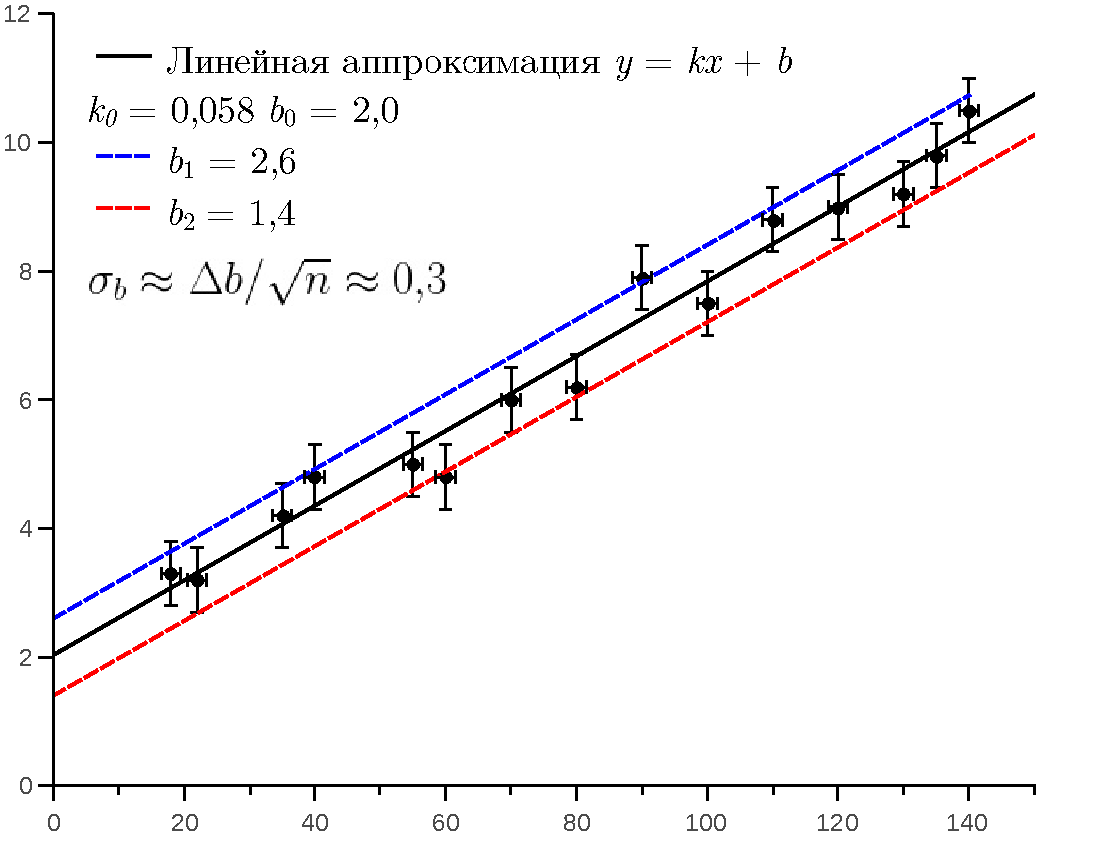
\includegraphics[width=1\linewidth,bb = 0 0 200 100, draft, type=eps]{График1.pdf}%
\end{minipage}%
\begin{minipage}[t]{0.5\columnwidth}%
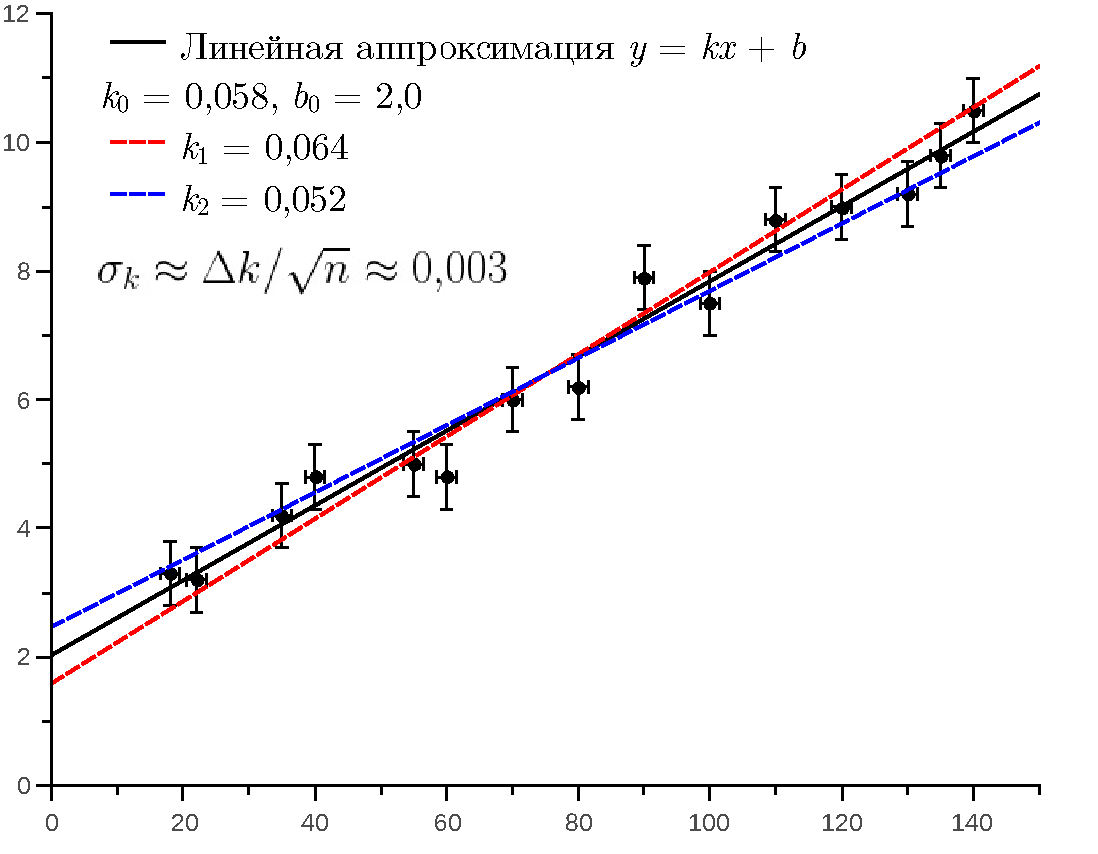
\includegraphics[width=1\linewidth,bb = 0 0 200 100, draft, type=eps]{График2.pdf}%
\end{minipage}

\caption{Графический метод проведения прямой и оценки погрешностей}
\end{figure}

Самый простой и грубый метод --- провести наилучшую прямую
<<на глазок>>. Этот метод, конечно, нестрогий,
но весьма наглядный. На практике к нему приходится часто прибегать
для грубой и быстрой оценки промежуточных результатов. Для этого нужно
приложить прозрачную линейку к графику так, чтобы по возможности кресты
всех экспериментальных точек находились максимально близко к проводимой
линии, а по обе стороны от неё оказалось примерно одинаковое количество
точек. 

Построив таким образом <<наилучшую>> прямую,
можно найти её параметры: угловой коэффициент $k$ и вертикальное
смещение $b$. Этим же способом можно грубо оценить ошибку определения
$k$ и $b$. Смещая линейку вертикально в пределах крестов погрешностей,
оценим погрешность $\delta b$. Аналогично, изменяя наклон линейки
относительно условного <<центра масс>>
экспериментального графика, получим оценку для погрешности углового
коэффициента $\delta k$. Если известно, что погрешности экспериментальных
точек $\left(\delta x,\,\delta y\right)$ имеют преимущественно случайный
характер, результат стоит разделить корень из числа точек: $\sigma_{k}\approx\delta k/\sqrt{n}$,
$\sigma_{b}\approx\delta b/\sqrt{n}$ (для систематических погрешностей
так делать не стоит).

Эта же процедура позволяет проверить, является ли измеренная зависимость
в самом деле линейной: прямая должна пересекать большую часть (хотя
бы 2/3) крестов погрешностей. В противном случае можно предполагать
существенное отклонение экспериментальной зависимости от линейной
теоретической. Отметим, что если кресты погрешностей на графике не
отмечены, такой анализ провести затруднительно. 

\textbf{\footnotesize{}Пример.}{\footnotesize{} На рис. TODO изображены
одни и те же экспериментальные точки при разных погрешностях измерений,
график 2а, несомненно, указывает на нерегулярный ход изучаемой зависимости
(кривая линия). Те же данные при больших погрешностях опыта (рис.
2б) успешно описываются прямой линией. То обстоятельство, что данные
на рис. 2а требуют проведения кривой линии, а на рис. 2б не требуют,
проясняется лишь при изображении результатов с крестами погрешностей.}{\footnotesize\par}

\paragraph{Нелинейные зависимости.}

Если теория предсказывает \emph{нелинейную }функциональную зависимость
между величинами, всегда можно сделать \emph{замену переменных} так,
чтобы результирующий график получался линейным.

\textbf{\footnotesize{}Пример.}{\footnotesize{} Высота и время падения
груза без начальной скорости в поле тяжести связаны соотношением $y=\frac{1}{2}gt^{2}+y_{0}$.
Для того, чтобы получить линейную зависимость, можно построить график
в координатах $\left(y,t^{2}\right)$. По угловому коэффициенту наилучшей
прямой можно в таком случае вычислить ускорение свободного падения:
$k=\frac{1}{2}g$.}{\footnotesize\par}

\textbf{\footnotesize{}Пример.}{\footnotesize{} В термодинамике и
химии часто встречается зависимость вида $y=Ce^{-a/x}$. Чтобы определить
коэффициенты $C$ и $a$, можно построить график в координатах $(u,v)$,
где $u=\ln y$ и $v=\frac{1}{x}$. В таком случае, как нетрудно видеть,
$u=-av+\ln C$.}{\footnotesize\par}

\subsection{Метод наименьших квадратов (МНК)\label{subsec:MNK}}
\todo[inline, author = Nozik]{Было очень много разговоров про погрешности, а после этого используется простой метод МНК, который их не использует. Для экономистов это нормально, но для физиков некорректно. Кроме того, не понятно, почему все излагается только для линейного случая. Думаю, что это надо переписать.}

Рассмотрим математически более строгий метод построения наилучшей
прямой $y=kx+b$ по набору экспериментальных точек 
\[
\left\{ \left(x_{i},y_{i}\right),i=1\ldots n\right\} .
\]

Расстояние от экспериментальной точки от искомой прямой, измеренное
по вертикали, равно
\[
\Delta y_{i}=y_{i}-\left(kx_{i}+b\right).
\]
Найдём такие коэффициенты $k$ и $b$, чтобы сумма квадратов таких
расстояний для всех точек была минимальной:
\begin{equation}
S\!\left(k,b\right)=\sum\limits _{i=1}^{n}\Delta y_{i}^{2}\to\mathrm{min}.\label{eq:mnk_S}
\end{equation}
Данный метод построения наилучшей прямой называют \emph{методом наименьших
квадратов} (МНК).

Рассмотрим сперва более простой частный случай. Пусть заведомо известно,
что искомая прямая проходит через ноль, то есть $b=0$ и $y=kx$.
Необходимое условие минимума функции $S\left(k\right)$, как известно,
есть равенство нулю её производной. Дифференцируя сумму (\ref{eq:mnk_S})
по $k$, считая все величины $\left\{ x_{i},\,y_{i}\right\} $ константами,
найдём 
\[
\frac{dS}{dk}=-\sum\limits _{i=1}^{n}2x_{i}\left(y_{i}-kx_{i}\right)=0.
\]
Решая относительно $k$, находим 
\[
k=\frac{\sum\limits _{i=1}^{n}x_{i}y_{i}}{\sum\limits _{i=1}^{n}x_{i}^{2}}.
\]
Поделив числитель и знаменатель на $n$, этот результат можно записать
более компактно:
\begin{equation}
\boxed{k=\frac{\left\langle xy\right\rangle }{\left\langle x^{2}\right\rangle }}.\label{eq:MNK0}
\end{equation}
Угловые скобки означают усреднение по всем экспериментальным точкам:
\[
\left\langle \ldots\right\rangle \equiv\frac{1}{n}\sum\limits _{i=1}^{n}\left(\ldots\right)_{i}
\]

В общем случае при $b\ne0$ функция $S\left(k,b\right)$ должна иметь
минимум как по $k$, так и по $b$. Поэтому имеем систему из двух
уравнений:
\begin{align*}
\frac{\partial S}{\partial k} & =-\sum\limits _{i=1}^{n}2x_{i}\left(y_{i}-kx_{i}-b\right)=0,\\
\frac{\partial S}{\partial b} & =-\sum\limits _{i=1}^{n}2\left(y_{i}-kx_{i}-b\right)=0.
\end{align*}
Решая систему, можно получить
\begin{equation}
\boxed{k=\frac{\left\langle xy\right\rangle -\left\langle x\right\rangle \left\langle y\right\rangle }{\left\langle x^{2}\right\rangle -\left\langle x\right\rangle ^{2}},\qquad b=\left\langle y\right\rangle -k\left\langle x\right\rangle }.\label{eq:MNK}
\end{equation}
Эти соотношения и есть решение задачи о построении наилучшей прямой
методом наименьших квадратов.

{\footnotesize{}Совсем кратко формулу (\ref{eq:MNK}) можно записать,
если ввести обозначение
\begin{equation}
D_{xy}\equiv\left\langle xy\right\rangle -\left\langle x\right\rangle \left\langle y\right\rangle =\left\langle \left(x-\left\langle x\right\rangle \right)\cdot\left(y-\left\langle y\right\rangle \right)\right\rangle \label{eq:cov}
\end{equation}
(в математической статистике $D_{xy}$ называют }\emph{\footnotesize{}ковариацией}{\footnotesize{};
при $x\equiv y$ имеем дисперсию $D_{xx}=\left\langle \left(x-\left\langle x\right\rangle \right)^{2}\right\rangle $).
Тогда
\begin{equation}
k=\frac{D_{xy}}{D_{xx}},\qquad b=\left\langle y\right\rangle -k\left\langle x\right\rangle .\label{eq:MNK_short}
\end{equation}
}{\footnotesize\par}

\paragraph{Погрешность МНК.}

Найдём погрешности $\sigma_{k}$ и $\sigma_{b}$ коэффициентов, вычисленных
по формуле (\ref{eq:MNK}) (или (\ref{eq:MNK0})).

Сделаем следующие предположения: погрешность измерений величины $x$
пренебрежимо мала: $\sigma_{x}\approx0$, а погрешность по $y$ одинакова
для всех экспериментальных точек $\sigma_{y}=\mathrm{const}$ и имеет
случайный характер (систематическая погрешность отсутствует).

Пользуясь в этих предположениях формулами для погрешностей косвенных
измерений (см. раздел (\ref{sec:kosv})) можно получить следующие
соотношения (выкладки здесь весьма громоздки, подробности можно найти
в п. (\ref{subsec:MMP})):
\begin{equation}
\sigma_{k}=\sqrt{\frac{1}{n-2}\left(\frac{D_{yy}}{D_{xx}}-k^{2}\right)},\label{eq:MNK_sigma}
\end{equation}
\begin{equation}
\sigma_{b}=\sigma_{k}\sqrt{\left\langle x^{2}\right\rangle },\label{eq:MNK_sigma_b}
\end{equation}
где использованы введённые выше сокращённые обозначения (\ref{eq:cov}).
Коэффициент $n-2$ отражает число независимых <<степеней
свободы>>: $n$ экспериментальных точек за вычетом двух
условий связи (\ref{eq:MNK}).

В частном случае $y=kx$ имеем
\begin{equation}
\sigma_{k}=\sqrt{\frac{1}{n-1}\left(\frac{\left\langle y^{2}\right\rangle }{\left\langle x^{2}\right\rangle }-k^{2}\right)}.\label{eq:MNK_sigma0}
\end{equation}


\paragraph{Условия применимости МНК.}

Формулы (\ref{eq:MNK}) (или (\ref{eq:MNK0})) позволяют провести
прямую по \emph{любому} набору экспериментальных данных, а формулы
(\ref{eq:MNK_sigma}) (или (\ref{eq:MNK_sigma0})) --- вычислить
соответствующую среднеквадратичную ошибку для её коэффициентов. Однако
далеко не всегда результат будет иметь физический смысл. Перечислим
ограничения применимости данного метода.

В первую очередь метод наименьших квадратов --- статистический,
и поэтому он предполагает использование достаточно большого количества
экспериментальных точек (желательно $n>10$).

Поскольку метод предполагает наличие погрешностей только по $y$,
оси следует выбирать так, чтобы погрешность $\sigma_{x}$ откладываемой
по оси абсцисс величины была минимальна.

Кроме того, метод предполагает, что все погрешности в опыте ---
случайны. Соответственно, формулы (\ref{eq:MNK_sigma}) и (\ref{eq:MNK_sigma0})
применимы \emph{только для оценки случайной составляющей} ошибки $k$
и $b$. Если в опыте предполагаются достаточно большие систематические
ошибки, они должны быть оценены \emph{отдельно}. Отметим, что для
оценки систематических ошибок не существует строгих математических
методов, поэтому в таком случае проще и разумнее всего воспользоваться
описанным выше графическим методом.

Наконец, стоит предостеречь от использования МНК <<вслепую>>,
без построения графика. Этот метод неспособен выявить такие <<аномалии>>,
как отклонения от линейной зависимости, немонотонность, случайные
всплески и т.п. Все эти случаи могут быть легко обнаружены при построении
графика и требуют особого рассмотрения.

Резюмируя, можно сформулировать универсальную практическую рекомендацию:
если результаты какого-либо математического метода обработки данных
существенно расходятся с тем, что можно получить <<вручную>>
графически, есть все основания сомневаться в применимости метода в
данной ситуации.

\subsection{Интерполяция и экстраполяция данных}

TODO

\subsection{Сглаживание и дифференцирование данных}

TODO

\section{Рекомендации по выполнению и представлению результатов работы}

\subsection{Проведение измерений}

\paragraph{Подготовка к работе.}

\begin{lyxgreyedout}
Перед выполнением учебной лабораторной работы необходимо
\begin{itemize}
\item ознакомиться с описанием работы и теоретическим введением по соответствующей
теме. Это необходимо, чтобы получить представление о явлениях, закономерностях
и порядках измеряемых величин, с которыми придётся иметь дело при
выполнении работы, а также о методе измерения и используемых приборах,
последовательности действий при проведении измерений;
\item для записей результатов работы надо подготовить рабочую тетрадь, лучше
большого формата, чтобы её можно было использовать в течение, по крайней
мере, одного семестра. Оформление каждой работы нужно начинать с номера
и названия. Далее должны быть представлены краткое изложение теории,
схема установки и описание хода эксперимента.
\item прежде чем приступить к выполнению работы, следует продумать предложенный
в описании план действий, определить необходимое количество измерений.
В соответствии с этим предварительно подготовить таблицы, в которые
будут заноситься результаты. 
\item желательно заранее представлять диапазон изменения измеряемых величин
и выбрать для них соответствующие единицы. В крайнем случае, это нужно
сделать на начальном этапе работы. 
\item необходимо подумать о точности измерений. Например, при косвенных
измерениях величин, имеющих степенную зависимость от непосредственно
измеряемых, относительная погрешность величин, входящих с б\'{о}льшими
показателями степени, должна быть меньше, то есть их следует измерять
точнее. По возможности следует избегать методов, при которых приходится
вычислять разность двух близких по значениям величин.
\end{itemize}
\end{lyxgreyedout}


\paragraph{Начало работы.}

\begin{lyxgreyedout}
В начале работы необходимо тщательно ознакомиться с экспериментальной
установкой, проверить работоспособность приборов. Нужно хорошо разобраться,
как они регулируются, включаются и выключаются.

Всегда очень важно аккуратное и бережное обращение с приборами. Не
следует вскрывать чувствительные приборы и менять настройку.

Все сведения о приборах (в первую очередь класс точности, максимальное
значение на шкале, по которой производятся измерения, и цену деления)
и условиях эксперимента необходимо записать в рабочей тетради, так
как они потребуются при получении окончательных результатов.

При составлении (собирании) электрических схем источники питания подключаются
к схеме в последнюю очередь.

Прежде чем приступить к основным измерениям, необходимо проверить
работу установки. Первые измерения должны быть контрольными, чтобы
убедиться, что все работает нормально, диапазон и точность измерений
выбраны правильно. Если разброс повторных измерений не превышает инструментальную
погрешность, то многократных измерений не требуется.

Замеченные неполадки в работе приборов и установок надо зафиксировать
(делать соответствующую запись в тетради) и сообщить об этом преподавателю.%
\end{lyxgreyedout}


\paragraph{Как выбрать число необходимых измерений.}

TODO

\paragraph{Проведение измерений.}

\begin{lyxgreyedout}
Все записи результатов измерений должны быть сделаны чётко и подробно,
с нужными пояснениями.

Полезно строить предварительные графики зависимостей измеряемых величин
между собой или от изменения параметров по мере получения результатов.
При этом сразу выделяются области резких изменений, в которых измерения
должны проводиться подробнее (больше точек), чем на участках плавного
изменения. Если изучаемая закономерность, например линейность, выполняется
только на некотором участке, то область измерений должна быть выбрана
шире этого участка, чтобы можно было установить границы выполнения
закономерности.

Если в начале работы выясняется, что разброс результатов измерений
очень большой, то иногда лучше поискать и устранить причину этого,
чем выполнять большое количество измерений для получения необходимой
точности результата. При изучении зависимости измеряемой величины
от параметра или другой измеряемой величины надо убедиться, что за
время измерений в процессе работы не произошло никаких сбоев или существенных
изменений внешних условий, влияющих на результаты, для чего в конце
работы необходимо повторить начальные измерения либо проделать все
измерения в обратном порядке.

Перед каждой таблицей должны быть указаны значения цены деления и
класс точности каждого прибора, которым производятся измерения. В
таблицу необходимо заносить число делений, а не саму величину, например,
тока или напряжения. Это убережёт вас от ошибки при записи экспериментальных
данных. В конечном счёте это главное, так как обработка данных может
быть проведена разными способами и в любое время, а измерения воспроизвести
бывает трудно, а иногда и невозможно.%
\end{lyxgreyedout}


\paragraph{Расчёты, анализ и представление результатов}

\begin{lyxgreyedout}
Полученные первичные результаты в виде таблиц и графиков используются
для расчёта конечных значений величин и их погрешностей либо для нахождения
зависимости измеряемых величин между собой. Все расчёты удобно проводить
в той же рабочей тетради, где записаны первичные результаты измерений,
и заносить в соответствующие свободные колонки таблиц с экспериментальными
данными. Это поможет проводить проверку, анализ и сопоставление получаемого
результата с исходными данными.

Для измеряемых величин окончательные результаты должны быть представлены
в виде среднего значения, погрешности и количества проведённых измерений.
В случае косвенных измерений для получения окончательного результата
используются их зависимости от измеряемых величин, по которым вычисляют
и средние значения и погрешности.

Для окончательной оценки качества полученных результатов измерений
надо сравнить их с данными, приводимыми в справочниках.%
\end{lyxgreyedout}


\subsection{Анализ инструментальных погрешностей}

Перед выполнением любого эксперимента необходимо предварительно проанализировать
возможные погрешности используемых приборов. Их погрешности могут
иметь как систематический, так и случайный характер. Можно говорить
о некоторой единой оценке \emph{инструментальной погрешности} прибора
$\sigma_{\text{инстр}}$, которая учитывает обе составляющие.

При работе с приборам \emph{со шкалой} (линейка, штангенциркуль, стрелочные
приборы и т.д.). один из источников погрешности~--- необходимость
выбора некоторого значения (интерполяции) между метками шкалы. Эта
погрешность, которую как правило оценивают в \emph{половину цены деления},
называется\emph{ погрешностью отсчёта} по шкале. Аналогичная погрешность
есть и у приборов с цифровым дисплеем --- это погрешность
округления цифры последнего разряда. Данная погрешность может быть
как случайной, так и систематической: в частности, если показания
прибора стабильны (стрелка не дрожит и при повторных измерения стрелка
попадает в то же самое место шкалы), ошибка отсчёта будет систематической;
если стрелка дрожит (или <<плавает>> последняя
цифра разряда), ошибка будет случайной. 

\textbf{\small{}Замечание.}{\small{} Отдельно отметим, что стоит по
возможности избегать измерений в начале шкалы: если измеряемая величина
лишь немногим превосходит цену деления (или единицу последнего разряда
дисплея), относительная ошибка измерения резко возрастает.}{\small\par}

Любой прибор имеет погрешность изготовления, калибровки, а также внутренние
источники ошибок (например, шумы). Как правило, максимальные значения
этих погрешностей определяются производителем и описаны в паспорте
прибора. Погрешности могут зависеть от условий эксплуатации (температура,
влажность и т.д.), что также должно отражаться в паспорте. 

\textbf{\footnotesize{}Пример.}{\footnotesize{} Согласно паспорту
вольтметра В7-34, его относительная погрешность при работе на пределе
измерений 1~В, оценивается по формуле 
\[
\varepsilon_{x}=\left[0{,}015+0{,}002\left(\frac{1\;\text{В}}{U_{x}}-1\right)\right]\cdot\bigr[1+0{,}01\cdot|t-20|\bigl],
\]
где $U_{x}$~{[}В{]} --- значение измеряемой величины,
$t$ {[}$^{\circ}\mathrm{C}${]}~--- комнатная температура.
Если измерения проводятся при температуре $24\;^{\circ}\mathrm{C}$
и прибор показывает напряжение $U_{x}=500\;\text{мВ}$, то относительная
погрешность равна $\varepsilon\approx1{,}7\%$, а абсолютная $\delta U\approx\pm8\;\text{мВ}.$}{\footnotesize\par}

Для стрелочных приборов традиционно используется понятие \emph{класса
точности}. Предельная инструментальная погрешность равна произведению
класса точности (в процентах) на показание прибора при максимальном
отклонении стрелки. В цифровых приборах погрешность, как правило,
зависит от диапазона измерения, поэтому понятие класса точности для
них не применяется.

\textbf{\footnotesize{}Пример.}{\footnotesize{} Стрелочный вольтметр
имеет диапазон измерения от 0 до 5~В и цену деления $10$~мВ, а
его класс точности равен $0{,}5$. Следовательно, погрешность измерения,
гарантируемая производителем, составляет $5\;\text{В}\cdot0{,}5\%=25$~мВ.
Хотя цена деления меньше, в качестве погрешности следует взять именно
$\pm25$ мВ. Не стоит рассчитывать на хорошую точность при измерениях
напряжения менее 1 В, поскольку относительная ошибка составит более
2,5\%.}{\footnotesize\par}

Наконец, при считывании показаний стрелка прибора или цифры на циферблате
могут <<дрожать>> (\emph{флуктуировать})
вблизи некоторого значения. Это может быть связано как с разного рода
шумами и помехами внутри прибора, так и с колебаниями самой измеряемой
величины. Если записывается некоторое среднее значение показаний,
то амплитуда флуктуаций должна быть учтена как дополнительная случайная
погрешность.

Не стоит также забывать, что в процессе эксперимента почти наверняка
возникнут дополнительные погрешности, связанные с конкретной постановкой
опыта и методикой измерений. Для нахождения результирующей погрешности
измерения необходимо сложить все \emph{независимые} источники ошибок
среднеквадратичным образом: $\sigma_{\text{полн}}=\sqrt{\sigma_{\text{инстр}}^{2}+\sigma_{\lyxmathsym{отсч}}^{2}+\sigma_{\text{случ}}^{2}+\ldots}$. 

\textbf{\small{}Замечание.}{\small{} Отметим, что цену деления шкалы
или разрядность дисплея }\emph{\small{}добросовестный}{\small{} производитель
выбирает таким образом, чтобы погрешность отсчёта и погрешность самого
прибора были согласованы. В таком случае погрешность отсчёта по шкале
отдельно учитывать не нужно --- она уже учтена производителем
при расчёте инструментальной погрешности.}{\small\par}

\begin{comment}
Несколько слов о точности линеек. Металлические линейки относительно
точны: миллиметровые деления наносятся с погрешностью не более $\pm0,05$~мм,
а сантиметровые не более чем с точностью 0,1~мм, так что считывание
результата измерения можно проводить с помощью лупы, снабжённой дополнительной
шкалой. Деревянными или пластмассовыми линейками лучше не пользоваться:
их погрешности неизвестны и могут оказаться неожиданно большими. Исправный
микрометр обеспечивает точность 0,01~мм, а погрешность измерения
штангенциркулем определяется точностью, с которой может быть сделан
отсчёт, т.~е. точностью нониуса. У штангенциркулей цена делений нониуса
составляет обычно 0,1 или 0,05~мм.
\end{comment}


\subsection{Оформление отчёта о работе}

Лабораторная работа студента --- миниатюрное научное исследование.
Настоящие требования основаны на общепринятых стандартах научных публикаций,
упрощенных для студентов младших курсов.

Отчёт о проделанной лабораторной работе должен представлять собой
целостный документ, позволяющий читателю получить максимально полную
информацию о проделанной работе и полученных результатах ---
без каких-либо дополнительных пояснений со стороны студента.

Материал в отчёте должен излагаться последовательно, а сам отчёт должен
быть структурирован по разделам. Отчёт, как правило, содержит разделы:
1) аннотация, 2) теоретические сведения, 3) методика измерений, 4)
используемое оборудование, 5) результаты измерений и обработка данных,
6) обсуждение результатов, 7) заключение. Структура и названия разделов
могут незначительно варьироваться в зависимости от конкретного содержания
работы.

Начальные разделы отчёта должны быть подготовлены \emph{до проведения
эксперимента} (при подготовке к работе). Непосредственно ход эксперимента
должен фиксироваться в отдельном лабораторном журнале студента. Записи
лабораторного журнала прикрепляются к отчёту в качестве приложения.
Допускается ведение лабораторного журнала и оформление отчётов в одной
рабочей тетради (формата А4).

Результаты измерений и сопутствующих вычислений должны быть представлены
в \emph{таблицах}. Таблицы должны иметь подписи с кратким описанием
их содержания и, возможно, с пояснениями по структуре расположения
данных. Заглавные столбцы (или строки) должны быть подписаны, в них
должны быть указаны буквенные обозначения величин (введенные в тексте
ранее) и их размерность. 

Размерность измеренных величин --- как в таблицах, так и
на графиках --- должна быть подобрана так, чтобы данные
были удобны для чтения и \emph{не содержали избыточное количество
нулей}.

Помимо таблиц и графиков в тексте отчёта также должны быть представлены
промежуточные результаты обработки данных (с соответствующими погрешностями),
указаны используемые методы обработки данных и приведены соответствующие
формулы. Окончательные и наиболее важные промежуточные результаты
должны быть записаны с указанием погрешности (как абсолютной, так
и относительной) и округлены согласно принятым в физике правилам округления.

\subsubsection*{Требования к содержанию разделов}
\begin{description}
\item [{Аннотация:}] краткое (1\textendash 2 абзаца) описание работы: её
цели, используемые методы и приборы, ожидаемые результаты.
\item [{Теоретические~сведения:}] краткий обзор основных понятий и теоретических
законов, используемых или проверяемых в работе; упрощения и предположения,
используемые при анализе и интерпретации результатов эксперимента;
основные расчётные формулы.
\item [{Методика~измерений:}] схема и описание экспериментальной установки;
краткое описание основных методик проведения эксперимента, получения
и обработки экспериментальных данных.
\item [{Используемое~оборудование:}] перечень измерительных приборов,
используемых в работе; инструментальные погрешности приборов и предварительный
анализ их влияния на результаты опыта.
\item [{Результаты~измерений~и~обработка~данных:}] результаты проведенных
измерений в форме таблиц и графиков; промежуточные и окончательные
расчёты, в том числе расчёт погрешностей полученных результатов.
\item [{Обсуждение~результатов:}] анализ точности проведённых измерений
и достоверности результатов; обсуждение применимости использованных
теоретических предположений; сравнение результатов с табличными (справочными)
данными или результатами других экспериментов; обсуждение возможных
причин ошибок и способов их устранения.
\item [{Заключение~(или~выводы):}] краткое резюме по результатам эксперимента:
что удалось или не удалось измерить, были ли достигнуты поставлены
цели, выводы по результатам работы и т.п.
\end{description}

\subsection{Правила округления\label{subsec:round}}

Запись числовых значений, полученных в результате измерений, отличается
от стандартной записи чисел, принятой в арифметике или в бухгалтерской
отчётности. При десятичной записи результата важно следить за тем,
какие цифры соответствуют реально измеренным в эксперименте, а какие
возникли исключительно в результате математических операций и находятся
за пределами точности опыта.

Все цифры, начиная с первой ненулевой, называют \emph{значащими}.
Для корректной записи результата необходимо следить, чтобы количество
значащих цифр было согласовано с погрешностью измерения. Перечислим
правила, которыми необходимо руководствоваться при записи результатов: 
\begin{itemize}
\item последняя цифра записи результата измерения должна соответствовать
тому же разряду, что и последняя цифра в погрешности:
\end{itemize}
\noindent%
\begin{tabular}{llll}
неправильно:  & $1{,}245\pm0{,}05$  & $5{,}2\pm0{,}36$  & $1{,}24\pm0{,}012$\tabularnewline
правильно:  & $1{,}25\pm0{,}05$  & $5{,}2\pm0{,}4$  & $1{,}240\pm0{,}012$ \tabularnewline
\end{tabular}
\begin{itemize}
\item величина погрешности имеет характер сугубо статистической \emph{оценки}
и практически \emph{не может быть определена с точностью лучше} 20\%.
Поэтому погрешность нужно округлять до \emph{одной\textendash двух
значащих цифр}. Как правило, если последняя цифра в погрешности единица
или двойка, в погрешности оставляют две значащие цифры, в остальных
случаях --- одну:
\end{itemize}
\noindent%
\begin{tabular}{llll}
неправильно:  & $5{,}27\pm0{,}86$  & $1{,}236\pm0{,}137$  & $1\pm0{,}239$\tabularnewline
правильно:  & $5{,}3\pm0{,}9$ & $1{,}24\pm0{,}14$ & $1{,}0\pm0{,}2$ или\tabularnewline
 &  &  & $1{,}00\pm0{,}24$\tabularnewline
\end{tabular}

\medskip{}

Величину $\pm0{,}14$ не следует округлять до $\pm0{,}1$, так как
при этом значение изменяется на 40\%.
\begin{itemize}
\item Ноль на конце десятичного числа является значащей цифрой. Запись $l=1{,}4$~м
не эквивалентна $l=1{,}40$ м, т.\,к. последняя подразумевает в 10
раз большую точность измерения. Например, не эквивалентны записи $m=1$~т
и $m=1000$~кг, так как в первом случае одна значащая цифра, а во
втором четыре.
\item При необходимости нужно пользоваться\emph{ научной} (или \emph{экспоненциальной})
формой записи числа, подбирая наиболее удобные единицы измерения.
Например, если длина объекта определена с точностью $\pm5$~см и
составляет $l=123\pm5$~см, то волне допустимы также записи: $l=1{,}23\pm0{,}05$~м,
или $l=\left(12{,}3\pm0{,}5\right)\cdot10^{-1}\;\text{м}$, или $l=\left(1{,}23\pm0{,}05\right)\cdot10^{3}\text{ мм}$,
и т.п. Не вполне корректно было бы написать $l=1230\pm50$~мм, поскольку
такая запись подразумевает превышение точности как в измеренной величине,
так и в оценке погрешности.
\item Если погрешность физической величины не указана, то по умолчанию подразумевается,
что она измерена с точностью до изменения последней значащей цифры
на единицу. Например, запись $l=1{,}23$~м эквивалентна $l=1{,}23\pm0{,}01$
м или $l=123\pm1$~см, но не эквивалентна $l=1230$~мм.
\end{itemize}
При записи \emph{промежуточных результатов} и в промежуточных вычислениях,
проводимых вручную, необходимо сохранять одну лишнюю значащую цифру,
чтобы избежать ненужных ошибок округления. При вычислениях на калькуляторе
необходимо следить, чтобы значащие цифры не вышли за пределы разрядности.
То же касается примитивных средств для обработки данных, таких как
электронные таблицы. Рекомендуется пользоваться только инженерными/научными
калькуляторами, которые не имеют ограничений по разрядности, а также
специализированными средствами обработки экспериментальных и статистических
данных.

\subsection{Построение графиков}

По возможности все основные результаты должны быть представлены в
виде \emph{графиков}. Основная цель использования графиков \textendash{}
\emph{наглядность} отображения результатов. В связи с этим к графикам
предъявляются следующие требования:
\begin{itemize}
\item график должен иметь подпись (заглавие) с кратким описанием его содержания;
подписи, данные и линии не должны быть нагромождены друг на друга
так, что препятствовало бы их чтению;
\item оси на графике должны быть \emph{подписаны}: указаны буквенное обозначение
величины и её единицы измерения; если величина безразмерна, указывается
<<отн. ед.>> (относительные единицы); 
\item на осях должны быть отмечены \emph{масштаб} и \emph{положение нуля};
масштаб обозначается несколькими отметками с подписанными значениями
и дополнительными малыми отметками без подписей; масштаб должен быть
удобным для чтения (использованы <<круглые>>
числа, делящиеся на 10, 5 или 2);
\item масштаб осей и начало отсчёта должны быть выбраны так, чтобы экспериментальные
данные занимали всю площадь листа, отведённую под график;
\item если график строится не <<от нуля>>, это
следует подчеркнуть отдельно, например <<разрывом>>
оси; 
\item при необходимости сравнения данных из разных серий измерений, их следует
размещать на одном графике, обозначая их разными символами или цветами; 
\item график с несколькими сериями данных должен быть снабжен <<легендой>>,
в которой указано соответствие серий данных и их обозначений; экспериментальные
<<точки>> должны изображаться \emph{символами
конечных размеров} (позволяющими отличить их от случайных <<пятен>>); 
\item точки не должны быть без необходимости соединены линиями; также не
нужно подписывать положение каждой точки графика (при необходимости
можно указать положение 1-2 \emph{особых} точек, если это не загромождает
график);
\item все экспериментальные точки должны быть снабжены \emph{крестами погрешностей},
размер которых соответствует инструментальной погрешности измерения
соответствующей величины (либо вычисленной по результатам косвенных
измерений); кресты погрешностей можно не отмечать, только если погрешности
малы (настолько, что они не будут видны на графике) или не известны; 
\item если теория предполагает некоторую (например, линейную) функциональную
зависимость, на график должна быть тонкой линией нанесена соответствующая
теоретическая кривая; расчёт параметров этой кривой (например, коэффициентов
МНК для линейной зависимости) должен проводиться отдельно в тексте
отчёта --- с указанием используемых методов и формул; результаты
таких расчётов и их погрешности указываются в легенде графика или
в подписи к нему;
\item оптимальный размер графика --- от четверти до половины страницы
(при условии, что отчёт оформляется на страницах формата А4).
\end{itemize}
На рис.~\ref{fig:incorrect} приведён пример того, как \emph{не надо}
строить графики. В нём собраны наиболее типичные ошибки, совершаемые
студентами. Предлагаем читателю выявить их самостоятельно. Для сравнения
на рис.~\ref{fig:correct} изображён график для \emph{тех же данных},
выполненный с соблюдением всех изложенных выше указаний.
\begin{figure}[H]
\begin{centering}
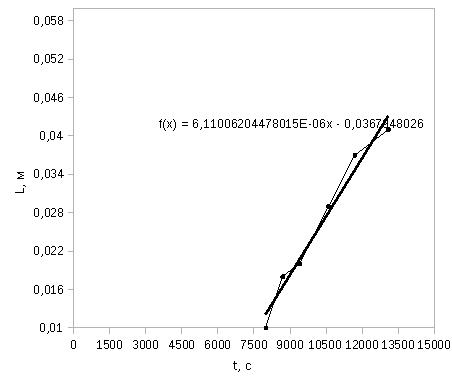
\includegraphics[width=8cm,bb = 0 0 200 100, draft, type=eps]{bad.png}
\par\end{centering}
\caption{\label{fig:incorrect}Пример неправильно построенного графика (график
построен с использованием электронных таблиц LibreOffice Calc)}
\end{figure}
\begin{figure}[H]
\begin{centering}
\includegraphics[width=7.5cm,bb = 0 0 200 100, draft, type=eps]{goog.pdf}
\par\end{centering}
\caption{\label{fig:correct}Пример корректного графического представления
данных (график построен с использованием специализированного приложения
для анализа и визуализации данных QtiPlot).}
\end{figure}


\subsection{Некоторые типичные ошибки обработки данных}

\paragraph{Нахождение углового коэффициента по среднему от частного.}

Студент измеряет сопротивление резистора по зависимости $U\!\left(I\right)$.
Получив некоторое количество экспериментальных точек $\left(I_{i},\,U_{i}\right)$,
и пользуясь законом Ома $R=U/I$, он вычисляет сопротивление для каждого
измерения $R_{i}=U_{i}/I_{i}$, а затем определяет сопротивление резистора
как среднее значение $R_{0}=\left\langle R_{i}\right\rangle =\frac{1}{n}\sum R_{i}$.
Что не так с этим методом (результат-то получается вполне разумным)?

{\footnotesize{}Во-первых, применять процедуру усреднения можно только
при повторении }\emph{\footnotesize{}одного и того же}{\footnotesize{}
измерения. В данном случае значения $R_{i}$ относятся к }\emph{\footnotesize{}разным}{\footnotesize{}
измерениям, так как параметры системы каждый раз изменялись. Во-вторых,
не была проверена линейность зависимости $U\left(I\right)$, то есть
справедливость закона Ома (ведь существуют и нелинейные элементы,
для которых закон Ома не выполняется). В-третьих, даже если зависимость
можно считать линейной, может оказаться так, что она не проходит через
ноль (например, из-за сдвига нуля у вольтметра или амперметра) ---
тогда нужно учитывать смещение и формула $R_{i}=U_{i}/I_{i}$ не годится.
И наконец, даже если выполнена линейность и зависимость проходит через
ноль, вычисление таким способом чревато большими погрешностями. Нетрудно
видеть, что среднее значение $\left\langle U_{i}/I_{i}\right\rangle $
по сути есть среднее тангенсов углов наклона линий, проведённых из
начала координат в экспериментальную точку (см. рис. TODO). Как известно,
функция $\tg x$ при $x>\pi/4$ очень резко возрастает (и стремится
к бесконечности при $x=\pi/2$). В таком случае даже небольшое <<шевеление>>
экспериментальной точки, особенно если она находится достаточно близко
к оси ординат, может привести к резкому увеличению вклада этой точки
в итоговый результат.}{\footnotesize\par}

{\footnotesize{}Таким образом, <<разумный>>
результат студента --- плод удачного стечения многих обстоятельств.
Правильный --- обоснованный и надёжный --- алгоритм
нахождения сопротивления: построить график $U\left(I\right)$, убедиться
в его линейности, и построить наилучшую прямую методом наименьших
квадратов. Угловой коэффициент этой прямой и будет наилучшей оценкой
для сопротивления резистора.}{\footnotesize\par}

\paragraph{Недооценка систематической погрешности.}

Студент измеряет сопротивление резистора, действуя по правильному
алгоритму, описанному выше. При измерениях используются вольтметр
и амперметр с классом точности $0{,}5$. Получив большое число экспериментальных
точек и построив наилучшую прямую методом наименьших квадратов (формула
(\ref{eq:MNK})), студент находит сопротивление (например, $R=5{,}555$~Ом)
и его погрешность по формуле (\ref{eq:MNK_sigma}), которая оказывается
равна $\sigma_{R}=0{,}003\;\text{Ом}.$ Окончательный результат измерения
записывается как $R=5{,}555\pm0{,}003\;\text{Ом}$.

Выходит так, что с помощью приборов, относительная погрешность которых
составляет $0{,}5\%$, получен на порядок более точный результат $\varepsilon\approx0{,}05\%$.
Возможно ли такое?

{\footnotesize{}Ситуация эта вполне реальна и встречается в учебной
лаборатории довольно часто. Дело в том, что метод наименьших квадратов
позволяет оценить }\emph{\footnotesize{}только случайную ошибку}{\footnotesize{}
--- и она в самом деле может оказаться довольно мала. Однако
учебные приборы далеки от совершенства и их ошибка имеет в основном
}\emph{\footnotesize{}систематический}{\footnotesize{} характер. Поэтому
в данном случае при записи конечного результата необходимо учесть
систематическую ошибку, относительная величина которой по составляет
не менее $0{,}5$\% (согласно классу точности прибора) и значительно
превосходит случайную. Результат эксперимента стоило бы записать как
$R=5{,}55\pm0{,}03\;\text{Ом}$.}{\footnotesize\par}

{\footnotesize{}Всё же, может статься и так, что инструментальные
ошибки наших вольтметра и амперметра имеют случайный характер, и мы
в самом деле добились кратного повышения точности за счёт многократных
повторений измерений (сколько нужно измерений, чтобы увеличить точность
на порядок?). Это нетрудно проверить, если заменить вольтметр или
амперметр на аналогичный и повторить опыты. Таким образом мы превратим
систематическую ошибку }\emph{\footnotesize{}одного}{\footnotesize{}
прибора в случайную ошибку }\emph{\footnotesize{}множества}{\footnotesize{}
приборов. Если отклонение нового результата от исходного значительно
превысит величину $\pm0{,}003$~Ом, гипотеза о случайности инструментальной
ошибки будет опровергнута, то есть погрешность отдельного прибора
действительно имеет в основном систематический характер.}{\footnotesize\par}

\paragraph{Аппроксимация полиномом.}

Студент получает набор экспериментальных данных $\left\{ x_{i},y_{i}\right\} $,
которые по теории должны ложиться на прямую. Нанеся точки на график,
студент видит, что на прямую они ложатся не очень хорошо (см. рис.~\ref{fig:approx}а).
Для того, чтобы точки лучше ложились на график, студент решает использовать
функцию аппроксимации полиномом (например, квадратичным), имеющуюся
в наличии во всех электронных таблицах и программах обработки данных.
Можно ли так делать?

\begin{figure}[h]
\begin{minipage}[t]{0.49\columnwidth}%
\begin{center}
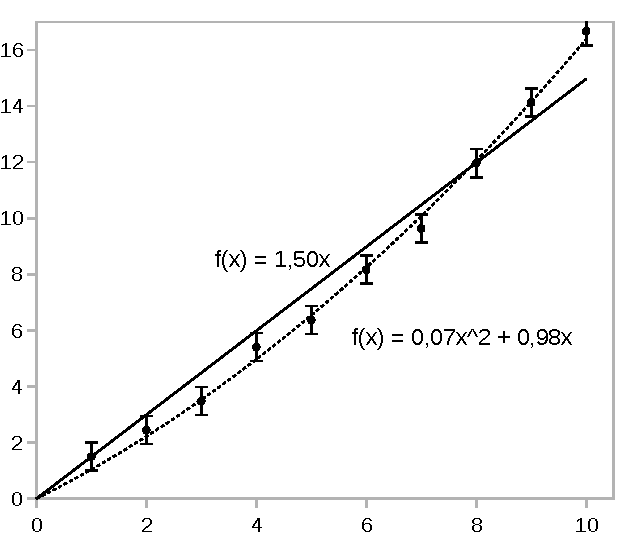
\includegraphics[width=1\linewidth,bb = 0 0 200 100, draft, type=eps]{x2.pdf}
\par\end{center}
\begin{center}
а)
\par\end{center}%
\end{minipage}%
\begin{minipage}[t]{0.49\columnwidth}%
\begin{center}
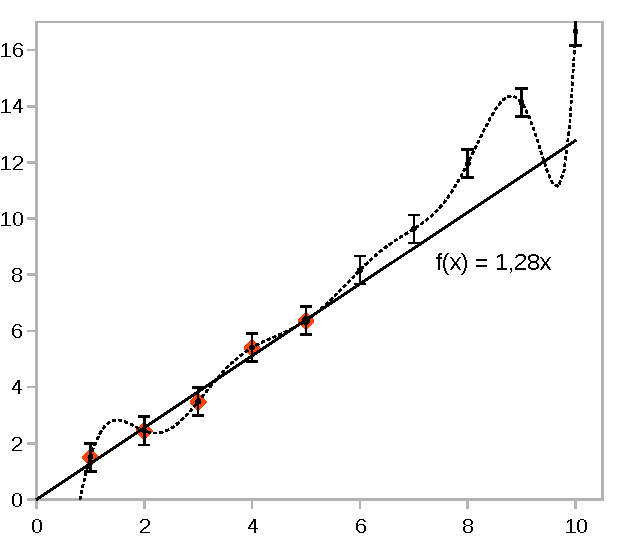
\includegraphics[width=1\linewidth,bb = 0 0 200 100, draft, type=eps]{x2b.pdf}
\par\end{center}
\begin{center}
б)
\par\end{center}%
\end{minipage}

\caption{\label{fig:approx}Примеры аппроксимации данных: а)~сплошная линия
\textendash{} линейная аппроксимация, пунктир --- квадратичная
аппроксимация; б)~сплошная линия --- линейная аппроксимация
по нескольким начальным точкам, пунктир --- аппроксимация
полиномом высокой степени.}
\end{figure}

{\footnotesize{}Ответ на вопрос зависит от того, какую цель преследует
студент. Если цель --- добиться того, чтобы <<точки
лучше ложились на график>>, то всё сделано правильно.
Если говорить <<по-научному>> ---
это попытка решить задачу }\emph{\footnotesize{}интерполяции}{\footnotesize{}
экспериментальных данных: по ограниченному набору $\left\{ x_{i},\,y_{i}\right\} $
получить аналитическую функцию $y=f\!\left(x\right)$, позволяющую
рассчитывать значения $y$ при произвольном $x$. В учебном практикуме
это может быть, например, задача построения калибровочного графика.
В таком случае можно лишь дать практический совет --- стараться
использовать для интерполяции полином }\emph{\footnotesize{}как можно
меньшей степени}{\footnotesize{} (дело в том, что при слишком большой
степени функция почти наверняка станет сильно немонотонной, а это
вовсе не то, что хочется иметь в качестве результата интерполяции,
см. рис.~\ref{fig:approx}б).}{\footnotesize\par}

{\footnotesize{}Однако ни в одной лабораторной работе курса общей
физики задача интерполяции не является основной целью работы! Как
правило, цель --- проверить теоретические закономерности
и измерить физические характеристики системы. Если нет теории, предсказывающей
и объясняющей квадратичную зависимость, проделанная студентом процедура
}\emph{\footnotesize{}бесполезна}{\footnotesize{}, поскольку вычисленным
коэффициентам полинома затруднительно приписать физический смысл. }{\footnotesize\par}

{\footnotesize{}Правильно было бы в такой ситуации выявить, на каком
участке зависимости линейный закон }\emph{\footnotesize{}выполняется}{\footnotesize{},
оценить его границы, и по нему построить наилучшую прямую (сплошная
линия на рис.~\ref{fig:approx}б). Для участка, отклоняющегося от
предсказываемой линей зависимости, следует теоретически проанализировать
причины отклонения и по возможности предложить уточнение теории. Возможно,
стоит ожидать не квадратичное, а кубическое отклонение? Различить
их на ограниченном наборе данных с большими погрешностями невозможно!
Имея достаточное количество точек предложенную теорию можно проверить
и лишь после этого аппроксимации более сложной функцией можно придать
физический смысл.}{\footnotesize\par}

\section{Дополнительные главы}

\subsection{{\small{}Принцип максимального правдоподобия и наилучшая оценка среднего}}

{\small{}Пусть при измерениях одно и той же величины два студента
независимым образом получили результаты 
\[
x_{1}\pm\sigma_{1}\qquad\text{и}\qquad x_{2}\pm\sigma_{2}.
\]
Можно ли как-то объединить их ответы и таким образом улучшить оценку
измеряемой величины?}{\small\par}

{\small{}Первое, что может прийти на ум --- найти среднее
арифметическое $\overline{x}=\frac{x_{1}+x_{2}}{2}.$ Однако нетрудно
понять, что если, скажем, измерение 2 сильно хуже, чем 1 ($\sigma_{2}\gg\sigma_{1}$),
то разумнее было бы значение $x_{2}$ вообще отбросить и использовать
$x_{1}$ как <<наилучшую>> оценку.}{\small\par}

{\small{}Предположим, что измеряемая величина имеет нормальное распределение
с некоторым средним $x_{0}$. Вероятность получить значение $x_{1}$
при первом измерении согласно (\ref{eq:normal}) пропорциональна величине
\[
P_{1}\propto\frac{1}{\sigma_{1}}e^{-\left(x_{1}-x_{0}\right)/2\sigma_{1}^{2}},
\]
вероятность получить значение $x_{2}$ при втором измерении:
\[
P_{2}\propto\frac{1}{\sigma_{2}}e^{-\left(x_{2}-x_{0}\right)^{2}/2\sigma_{2}^{2}}.
\]
Вероятность получить пару значений $\left\{ x_{1},\,x_{2}\right\} $
пропорциональна произведению $P_{1}P_{2}$:
\[
P\left(x_{1},x_{2}\right)=P_{1}P_{2}\propto\frac{1}{\sigma_{1}\sigma_{2}}e^{-\left(x_{1}-x_{0}\right)^{2}/2\sigma_{1}^{2}-\left(x_{2}-x_{0}\right)^{2}/2\sigma_{2}^{2}}.
\]
}{\small\par}

{\small{}Рассмотрим выражение, оказавшееся в показателе экспоненты:
\[
\chi^{2}=\left(\frac{x_{1}-x_{0}}{\sigma_{1}}\right)^{2}+\left(\frac{x_{2}-x_{0}}{\sigma_{2}}\right)^{2}.
\]
}{\small\par}

{\small{}Назовём }\emph{\small{}наилучшей}{\small{} такую оценку параметра
$x_{0}$, при котором полученные в опытах результаты имеют }\emph{\small{}максимальную
вероятность}{\small{} ($P\to\mathrm{max}$). Такой подход, называемый
}\emph{\small{}принципом максимального правдоподобия}{\small{}, используется
во многих задачах статистики.}{\small\par}

{\small{}Из полученного выше видно, что $P\to\mathrm{max}$, если
величина $\chi^{2}$ (}\emph{\small{}хи-квадрат}{\small{}) будет иметь
}\emph{\small{}минимум}{\small{}. Дифференцируя по $x_{0}$ и приравнивая
результат к нулю, запишем 
\[
\frac{d\chi^{2}}{dx_{0}}=-2\frac{x_{1}-x_{0}}{\sigma_{1}^{2}}-2\frac{x_{2}-x_{0}}{\sigma_{2}^{2}}=0,
\]
откуда найдём
\begin{equation}
x_{0}=\frac{w_{1}x_{1}+w_{2}x_{2}}{w_{1}+w_{2}},\qquad\text{где }w_{1,2}=\frac{1}{\sigma_{1,2}^{2}}.
\end{equation}
}{\small\par}

{\small{}Таким образом, для вычисления}\emph{\small{} наилучшей (максимально
правдоподобной) }{\small{}оценки среднего нужно вычислить }\emph{\small{}взвешенное
среднее}{\small{} с весами, }\emph{\small{}обратно пропорциональными
квадратам соответствующих погрешностей}{\small{}.}{\small\par}

{\small{}Результат непосредственно обобщается на произвольное число
измерений:
\begin{equation}
x_{\text{наил}}=\frac{\sum\limits _{i}w_{i}x_{i}}{\sum\limits _{i}w_{i}},\qquad w_{i}=\sigma_{i}^{-2}.
\end{equation}
}{\small\par}

\subsection{{\normalsize{}Метод максимального правдоподобия для построения наилучшей
прямой\label{subsec:MMP}}}

{\small{}При описании метода наименьших квадратов мы не обосновали,
почему и в каком смысле именно этот метод является <<наилучшей>>
оценкой для коэффициентов линейной регрессии $y=kx+b$. Кроме того,
мы получили формулы только для частного случая, когда погрешности
всех экспериментальных точек одинаковы: $\sigma_{y}=\mathrm{const}$.}{\small\par}

{\small{}Рассмотрим более общий случай. Пусть по-прежнему погрешности
по оси абсцисс малы, $\sigma_{x}\to0$, а погрешности по оси $y$
различны для каждой точки и равны $\sigma_{y_{i}}$. Пусть теория
предсказывает }\emph{\small{}линейную}\footnote{{\footnotesize{}Отметим, что метод легко обобщается и на нелинейные
зависимости общего вида $y=f\left(x;a,b,\ldots\right)$. Хотя формулы
получаются существенно более громоздкими, при вычислении на компьютере
оперировать с ними не сложнее, чем с линейной регрессией. В учебном
практикуме мы рекомендуем всегда делать замену переменных, сводящую
теоретическую зависимость к линейной, поскольку проведение прямой
наиболее наглядно и может быть в грубом приближении проделано просто
<<по линейке>>.}}{\small{} зависимость $y=kx+b$.}{\small\par}

{\small{}Отклонение точки от теоретической зависимости обозначим как
\[
\Delta y_{i}=y_{i}-\left(kx_{i}+b\right).
\]
}{\small\par}

{\small{}Воспользуемся }\emph{\small{}принципом максимального правдоподобия}{\small{}
и построим такую прямую, чтобы вероятность обнаружить наблюдаемые
в опыте отклонения $\left\{ \Delta y_{i}\right\} $ от неё была максимальна.}{\small\par}

{\small{}Обозначим вероятность отклонения на величину $\Delta y_{i}$
при известном $\sigma_{y_{i}}$ как $P\!\left(\Delta y_{i};\sigma_{y_{i}}\right)$.
Предположим, что ошибки измерения для всех экспериментальных точек
можно считать }\emph{\small{}случайными}{\small{} и }\emph{\small{}независимыми}{\small{}.
В таком случае вероятность отклонения для всех $n$ точек равна произведению
вероятностей, так что метод максимального правдоподобия сводится к
поиску максимума выражения
\begin{equation}
\prod\limits _{i=1}^{n}P\!\left(\Delta y_{i};\sigma_{y_{i}}\right)\to\mathrm{max}.\label{eq:MMP_general}
\end{equation}
Максимизация производится по параметрам аппроксимирующей функции (на
нашем случае это $k$ и $b$).}{\small\par}

{\small{}Рассмотрим частный случай, когда погрешности имеют }\emph{\small{}нормальное}{\small{}
(гауссово) распределение (\ref{eq:normal}) (напомним, что нормальное
распределение применимо, если отклонения возникают из-за большого
числа независимых факторов, что на практике реализуется довольно часто).
Тогда, поскольку гауссова функция распределения пропорциональна величине
$\propto e^{-\Delta y^{2}/2\sigma^{2}}$, выражение (\ref{eq:MMP_general})
достигает максимума, если минимальна сумма
\begin{equation}
\boxed{\chi^{2}=\sum_{i=1}^{n}\frac{\Delta y_{i}^{2}}{\sigma_{y_{i}}^{2}}\to\mathrm{min}}.\label{eq:chi2}
\end{equation}
Здесь мы ввели стандартное обозначение для такой суммы ---
$\chi^{2}$ (}\emph{\small{}хи-квадрат}{\small{}).}{\small\par}

{\small{}Таким образом, задача построения наилучшей прямой сводится
к минимизации суммы квадратов отклонений, нормированных на соответствующие
дисперсии $\sigma_{y_{i}}^{2}$. Если все погрешности одинаковы, $\sigma_{y_{i}}=\mathrm{const}$,
мы приходим к методу наименьших квадратов.}{\small\par}

{\small{}Получим выражения для наилучших коэффициентов $k$ и $b$.
Заметим, что сумма (\ref{eq:chi2}) является }\emph{\small{}взвешенной}{\small{}
суммой квадратов отклонений с весами
\begin{equation}
w_{i}=\frac{1}{\sigma_{y_{i}}^{2}}.
\end{equation}
}{\small\par}

{\small{}Можно определить }\emph{\small{}взвешенное среднее }{\small{}от
некоторого набора значений $\left\{ x_{i}\right\} $ как
\[
\left\langle x\right\rangle ^{\prime}=\frac{1}{W}\sum_{i}w_{i}x_{i},
\]
где $W=\sum\limits _{i}w_{i}$ --- нормировочная константа.
Далее в этом разделе штрих будем для краткости опускать.}{\small\par}

{\small{}Потребуем, согласно (\ref{eq:chi2}), чтобы была минимальна
сумма
\[
\sum\limits _{i=1}^{n}w_{i}\Delta y_{i}^{2}\to\mathrm{min}.
\]
Повторяя процедуру, использованную при выводе (\ref{eq:MNK}), можно
получить совершенно аналогичные формулы для оптимальных коэффициентов:
\begin{equation}
\boxed{k=\frac{\left\langle xy\right\rangle -\left\langle x\right\rangle \left\langle y\right\rangle }{\left\langle x^{2}\right\rangle -\left\langle x\right\rangle ^{2}},\qquad b=\left\langle y\right\rangle -k\left\langle x\right\rangle },\label{eq:MMP}
\end{equation}
с тем отличием, что под угловыми скобками $\left\langle \ldots\right\rangle $
теперь надо понимать усреднение с весами $w_{i}=1/\sigma_{y_{i}}^{2}$.}{\small\par}

{\small{}Найденные формулы позволяют вычислить коэффициенты линейной
регрессии, }\emph{\small{}если}{\small{} известны величины $\sigma_{y_{i}}$.
Значения $\sigma_{y_{i}}$ могут быть получены либо из некоторой теории,
либо измерены непосредственно (многократным повторением измерений
при каждом $x_{i}$), либо оценены из каких-то дополнительных соображений
(например, как инструментальная погрешность).}{\small\par}

\paragraph{{\small{}Погрешности коэффициентов.}}

{\small{}Проведём подробный вывод для погрешностей коэффициентов наилучшей
прямой $\sigma_{k}$ и $\sigma_{b}$. Воспользуемся общей формулой
(\ref{eq:sigma_general}) для погрешности косвенных измерений. Считая,
что величины $x_{i}$ известны точно, запишем для погрешности углового
коэффициента
\[
\sigma_{k}^{2}=\sum\limits _{i}\left(\frac{\partial k}{\partial y_{i}}\right)^{2}\sigma_{y_{i}}^{2}.
\]
Продифференцируем (\ref{eq:MMP}) по $y_{i}$:
\[
\frac{\partial k}{\partial y_{i}}=\frac{1}{D_{xx}}\frac{\partial}{\partial y_{i}}\left(\frac{1}{W}\sum w_{i}x_{i}y_{i}-\left\langle x\right\rangle \frac{1}{W}\sum w_{i}y_{i}\right)=\frac{w_{i}\left(x_{i}-\left\langle x\right\rangle \right)}{WD_{xx}},
\]
где $D_{xx}=\left\langle x^{2}\right\rangle -\left\langle x\right\rangle ^{2}=\left\langle (x-\left\langle x\right\rangle )^{2}\right\rangle $.
Тогда
\[
\sigma_{k}^{2}=\frac{1}{W^{2}D_{xx}^{2}}\sum\limits _{i}w_{i}^{2}\left(x_{i}-\left\langle x\right\rangle \right)^{2}\sigma_{y_{i}}^{2}.
\]
Учитывая, что $w_{i}\sigma_{y_{i}}^{2}=1$, получим
\begin{equation}
\boxed{\sigma_{k}^{2}=\frac{1}{D_{xx}\cdot\sum\limits _{i}\sigma_{y_{i}}^{-2}}}.\label{eq:MMP_sigma_k}
\end{equation}
}{\small\par}

{\small{}Аналогично, для погрешности свободного члена имеем
\[
\sigma_{b}^{2}=\sum_{i}\left(\frac{\partial b}{\partial y_{i}}\right)^{2}\sigma_{y_{i}}^{2},
\]
где 
\[
\frac{\partial b}{\partial y_{i}}=\frac{w_{i}}{W}+\frac{\partial k}{\partial y_{i}}\left\langle x\right\rangle =\frac{w_{i}}{W}\left(1-\frac{x_{i}-\left\langle x\right\rangle }{\left\langle x^{2}\right\rangle -\left\langle x\right\rangle ^{2}}\left\langle x\right\rangle \right)=\frac{w_{i}}{W}\frac{\left\langle x^{2}\right\rangle -x_{i}\left\langle x\right\rangle }{D_{xx}}.
\]
Отсюда, пользуясь (\ref{eq:MMP_sigma_k}), приходим к формуле (\ref{eq:MNK_sigma_b}):
\[
\sigma_{b}^{2}=\sigma_{k}^{2}\frac{\left\langle \left(\left\langle x^{2}\right\rangle -x\left\langle x\right\rangle \right)^{2}\right\rangle }{\left\langle x^{2}\right\rangle -\left\langle x\right\rangle ^{2}}=\sigma_{k}^{2}\left\langle x^{2}\right\rangle .
\]
}{\small\par}

\paragraph{{\small{}Случай $\sigma_{y}=\mathrm{const}$.}}

{\small{}В частном случае, расмотренном в п. (\ref{subsec:MNK}),
формула (\ref{eq:MMP_sigma_k}) упрощается:
\begin{equation}
\boxed{\sigma_{k}^{2}=\frac{\sigma_{y}^{2}}{nD_{xx}},\qquad\sigma_{b}^{2}=\sigma_{k}^{2}\left\langle x^{2}\right\rangle }.\label{eq:MMP_sigma_k_simple}
\end{equation}
Здесь величина $\sigma_{y}$ может быть оценена непосредственно из
экспериментальных данных:
\begin{equation}
\sigma_{y}\approx\sqrt{\frac{1}{n-2}\sum_{i}\Delta y_{i}^{2}},\label{eq:MMP_sigma_y}
\end{equation}
где $n-2$ --- число <<степеней свободы>>
для приращений $\Delta y_{i}$ ($n$ точек за вычетом двух связей
(\ref{eq:MMP})).}{\small\par}

{\small{}Формул (\ref{eq:MMP_sigma_k_simple}) и (\ref{eq:MMP_sigma_y}),
вообще говоря, достаточно для вычисления погрешности величины $k$
по известным экспериментальным точкам. Однако часто их объединяют
в одно упрощённое выражение. Для этого преобразуем (\ref{eq:MMP_sigma_y})
следующим образом: учитывая, что $\left\langle y\right\rangle =k\left\langle x\right\rangle +b$,
запишем 
\[
\Delta y_{i}=y_{i}-kx_{i}-b=\left(y_{i}-\left\langle y\right\rangle \right)-k\left(x_{i}-\left\langle x\right\rangle \right).
\]
Возведём в квадрат, усредним и воспользуемся выражением для $k$ в
форме (\ref{eq:MNK_short}):
\[
\left\langle \Delta y^{2}\right\rangle =D_{yy}+k^{2}D_{xx}-2kD_{xy}=D_{yy}-k^{2}D_{xx}.
\]
Таким образом, 
\[
\sigma_{y}=\sqrt{\frac{n}{n-2}\left(D_{yy}-k^{2}D_{xx}\right)},
\]
и с помощью (\ref{eq:MMP_sigma_k_simple}) получаем формулы (\ref{eq:MNK_sigma}),
(\ref{eq:MNK_sigma_b}):
\[
\boxed{\sigma_{k}=\sqrt{\frac{1}{n-2}\left(\frac{D_{yy}}{D_{xx}}-k^{2}\right)},\qquad\sigma_{b}=\sigma_{k}\sqrt{\left\langle x^{2}\right\rangle }}.
\]
}{\small\par}

\subsection{{\small{}Проверка гипотез}}

{\small{}Предположим, что теория предсказывает некоторую зависимость
\[
y=f\!\left(x;a,b,\ldots\right),
\]
а в эксперименте получен набор значений $\left\{ x_{i},\,y_{i}\right\} $.
Метод максимального правдоподобия позволяет получить параметры $\left\{ a,b,\ldots\right\} $
функции $f$, <<наилучшим>> образом приближающие
экспериментальные значения. Причём, как бы плохо экспериментальные
точки не ложились на теоретическую кривую, ответ будет получен в любом
случае. Как проверить, действительно ли измеряемые величины можно
считать связанными зависимостью $y=f\!\left(x\right)$?}{\small\par}

{\small{}Задача может быть решена, если, как обычно, сделать ряд упрощающих
предположений}\footnote{{\small{}Отметим, что в общем случае такая проверка не осуществима:
в частности, если погрешности экспериментальных точек велики или не
известны, то через них с равным <<успехом>>
можно провести почти }\emph{\small{}любую}{\small{} функцию!}}{\small{}. Пусть опять все ошибки измерения }\emph{\small{}независимы}{\small{},
распределены }\emph{\small{}нормально }{\small{}и нам известны их
среднеквадратичные значения $\sigma_{y_{i}}$ (или хотя бы их грубые
оценки).}{\small\par}

{\small{}Рассмотрим определённую выше сумму }\emph{\small{}хи-квадрат}{\small{}
(\ref{eq:chi2}) как функцию $n$ переменных $\left\{ y_{i}\right\} $:
\begin{equation}
\chi^{2}\!\left(y_{1},\,y_{2},\,\ldots,\,y_{n}\right)=\sum\limits _{i=1}^{n}\left(\frac{y_{i}-f\!\left(x_{i}\right)}{\sigma_{y_{i}}}\right)^{2}.\label{eq:chi2-1}
\end{equation}
Пусть функция $f\!\left(x\right)$ содержит $p$ <<подгоночных>>
параметров (например, $p=2$ для линейной зависимости $f\!\left(x\right)=kx+b$).
Найдём их наилучшие значения по методу максимального правдоподобия
($\chi^{2}\to\mathrm{min}$), и зафиксируем их. После этого $\chi^{2}$
можно рассматривать как функцию 
\[
m=n-p
\]
 независимых переменных. Величину $m$ назовём }\emph{\small{}числом
степеней свободы}{\small{} задачи}\emph{\small{}.}{\small\par}

{\small{}Попробуем сперва качественно ответить на вопрос, какое значение
величины $\chi^{2}$ можно ожидать, если зависимость $y=f\!\left(x\right)$
справедлива? Ясно, что если распределение ошибок нормальное, можно
ожидать отклонений порядка среднеквадратичного: $\Delta y_{i}=y_{i}-f\!\left(x_{i}\right)\sim\sigma_{y_{i}}$.
Поэтому значение суммы (\ref{eq:chi2-1}) должно оказаться порядка
числа входящих в неё независимых слагаемых: $\chi_{m}^{2}\sim m$.
В теории вероятностей доказывается}\footnote{См., например, \emph{Д. Худсон} Статистика для физиков. ---
М. Мир, 1970.}{\small{}, что ожидаемое среднее значение (математическое ожидание)
$\chi^{2}$ в точности равно числу степеней свободы: $\overline{\chi_{m}^{2}}=m$.}{\small\par}

{\small{}Теперь можно сформулировать качественный критерий проверки
гипотезы о наличии некоторой функциональной зависимости (его называют
}\emph{\small{}критерий хи-квадрат}{\small{}): }{\small\par}
\begin{itemize}
\item {\small{}если $\chi^{2}\sim m$, согласие эксперимента с теорией }\emph{\small{}удовлетворительное}{\small{}
(гипотеза не опровергнута); }{\small\par}
\item {\small{}если $\chi^{2}\gg m$ --- }\emph{\small{}согласия
нет}{\small{}, то есть гипотеза о зависимости скорее всего $y=f\!\left(x\right)$
не верна.}{\small\par}
\end{itemize}
{\small{}Заметим, что если вдруг $\chi^{2}\ll m$, то совпадение }\emph{\small{}слишком}{\small{}
хорошее, и скорее всего имеет место завышенная оценка для случайных
погрешностей измерения $\sigma_{y_{i}}$.}{\small\par}

{\small{}Для того, чтобы дать строгий }\emph{\small{}количественный}{\small{}
критерий, с какой долей вероятности гипотезу $y=f\!\left(x\right)$
можно считать подтверждённой или опровергнутой, нужно детально исследовать
вероятностный закон, которому подчиняется функция $\chi^{2}$. В теории
вероятностей он называется }\emph{\small{}распределение хи-квадрат}{\small{}
(с $m$ степенями свободы). В элементарных функциях распределение
хи-квадрат не выражается, но может быть легко найдено численно: функция
встроена во все основные статистические пакеты, либо может быть вычислена
по таблицам. Как правило, определяется вероятность $P\left(\chi^{2}>\chi_{0}^{2}\right)$
того, что хи-квадрат имеет значение больше некоторого $\chi_{0}^{2}$,
вычисленного из эксперимента. Если эта вероятность достаточно мала
(например, $P<5\%$; конкретная величина доверительной вероятности
всегда остаётся на усмотрение исследователя), соответствующую гипотезу
следует признать несостоятельной.}{\small\par}

\textbf{\footnotesize{}Пример.}{\footnotesize{} Для данных на рис.~\ref{fig:correct}
при $\sigma_{y}=0{,}2$ см величина хи-квадрат равна $\chi^{2}\approx4{,}7$.
За вычетом двух параметров линейной аппроксимации имеем $m=6-2=4$
степеней свободы. По графику TODO определяем, что вероятность того,
что согласие окажется хуже, чем на TODO (т.е. разброс точек относительно
}\emph{\footnotesize{}той же}{\footnotesize{} прямой будет больше),
составляет $P\sim30\%$. Оснований для отказа от <<гипотезы
о линейной зависимости>> нет.}{\footnotesize\par}

{\footnotesize{}Если бы погрешность каждой точки была равна $\sigma_{y}=0{,}14$
см, то мы получили бы $\chi^{2}=9{,}7$. Это соответствует $P<5\%$,
так что считать зависимость линейной, по-видимому, было бы нельзя
(либо не верна оценка для погрешности $\sigma_{y}$).}{\footnotesize\par}

{\small{}Напоследок еще раз подчеркнём, что критерий хи-квадрат, во-первых,
статистический и не может дать однозначного ответа --- только
вероятностную оценку, а во-вторых, он работает корректно при условии,
что ошибки разных точек независимы и каждая имеет нормальное распределение.
Эти предположения, вообще говоря, выполняются далеко не всегда и,
по-хорошему, требуют отдельной проверки.}{\small\par}
\begin{thebibliography}{1}
\bibitem{taylor}Тейлор

\bibitem{squires}Сквайрс

\bibitem{zaidel}Зайдель

\bibitem{hudson}Худсон
\end{thebibliography}

\end{document}
